\chapter{Style Extraction and Transfer}
\minitoc% Creating an actual minitoc

\par We finally arrive to the core objective of the PhD: how to leverage information of style from one (or more) \Gls{task}/s, in order to bootstrap the learning of a new task?


\section{Introduction and objectives}
  % \begin{itemize}
  %     \item Explain different paradigms and metrics used to characterise transfer learning.
  %     \item Why extracting style?: on our side, as ML practitioners, the ultimate objective of using ML is to help us extract new knowledge
  %     \item The questions of research here: extracting styles from bottleneck, transfer between writers, transfer between tasks
  % \end{itemize}

  \par Before we dive into the technical details, it is important to motivate why do we need to perform this in the first place. A common scenario is that we collect data over time for a particular task. This process can be quite expensive (e.g., collecting data from the robots is a slow and expensive process). Then, a new task of interest emerges. This task has common aspects with the old one. The question here is if we can leverage this common aspects, in order to boostrap the learn the new task.

  % For example, in case of handwriting, when trying to write new letters, and need to have the skill of using the pen, and performing micro-actions, like curves and straight lines. In the case of new letters, we need to recombine those mico-actions with new actions, in order to draw the new letters. Another example, in case of humans, is grasping objects. If you learn how to hold a plastic bottle, then you try to hold a glass cup, there are a lot of atomic actions in common, but the forces you apply are different.

  \par Examples of transfer learning:
  \begin{itemize}
      \item If you know how to hold a glass cup, with little adjustments, you can learn how to hold a plastic bottle.
      \item If you know probability and algebra, you can use this knowledge in order to boostrap/accelerate your progress in mastering machine learning.
  \end{itemize}

  \par There are plenty of cases where transfer learning is/could be useful, like:
  \begin{itemize}
    \item In robotics \citep{konidaris2012robot,Konidaris:2012:TRL:2188385.2343689}, collecting data can be quite expensive process, due to hardware limitations from one side, and human limitatio as well (in case of human-robot interaction scenarios). In addition, with techniques like reinforcement learning \citep{sutton2018reinforcement}, where the agent learns by trial and error, the process can be prohibitively slow, with safety concerns sometimes.
    \item In underwater acoustics \citep{malfante2018automatic}, an essential task is collecting and cleaning the data about the different fish sounds. This is a tediously manual job, and any change (type of fish, time of the day or place in the ocean) degrades the quality of prediction a lot. Transfer learning can be very useful in this case, to reduce the effort needed to collect, clean and annotate the data.
  \end{itemize}

  \begin{mdframed}[backgroundcolor=blue!20]
      \begin{center}
          Points addressed in this chapter
      \end{center}

      \begin{itemize}
          \item What is transfer learning? and what are the different approaches to perform it? I will explain the different paradigms and metrics used to characterise transfer learning.
          \item How do we approach the problem of style transfer, for both handwriting and sketch drawing?
          \item The experiments performed, the results, and our conclusions.
      \end{itemize}
  \end{mdframed}

\section{Transfer learning}\label{sec:transfer_learning}
  \par An important research direction in machine learning nowadays is transfer learning. If humans and machines are able to learn how to perform a task, one of the thing that separates humans from machines is the ability to leverage this knowledge in order to acquire new skills and perform new tasks, without the need for additional trials and errors from tabula rasa. This however, is not a straightforward thing for machine learning to do. The algorithms are fitted to data responding directly to the task required (i.e., has the same input feature space and same distribution). Thus, a change in the task can lead to degradation in the algorithm performance \citep{shimodaira2000improving,pan2009survey,weiss2016survey,dtl2018survey}.

  % \par In the following subsections, I first introduced notations and clear description for the objective of transfer learning, and the metrics used to evaluate the quality of transfer. I then discuss different types of transfer learning, with examples on each type.

  % \subsection{Notation and problem definition}
  \par Let's first introduce some notations that will help in formulating the problem:
  \begin{itemize}
      \item We first introduce the concept of \textit{Domain}. A domain defines a feature space (e.g., images of animals), and the probability distribution of this space (i.e., the distribution of pixels in the images of animals). We can consider the domain as the available \textit{knowledge} to us. Thus, a domain $\mathcal{D}$ is defined as $\mathcal{D} = \{\mathcal{X}, P(X)\}$, where:\\
      $\mathcal{X}$ is the feature space, $X$ is the data samples available to us from the feature samples, $X = \{x_1,x_2,\cdots,x_n\} \in \mathcal{X}$, where $n$ is the size of the learning sample. $P(X)$ is the marginal distribution probability of this data sample.

      \item For a given domain (aka, the knowledge available to us), we define a the concept of a \textit{task}. A task is something we would like to achieve using the knowledge we have. For example, a task can be classifying animals given animal pictures, or perform robot navigation given a map of the building. Thus, a task $\mathcal{T}$ is defined as $\mathcal{T} = \{\mathcal{Y}, f(.)\}$, where:\\
      $\mathcal{Y}$ is the label space (the task objectives), $f(.)$ is the mapping function (mapping the domain knowledge to the task objectives). It can also be rewritten as a conditional probability over the domain knowledge, $\mathcal{T} = \{\mathcal{Y}, P(Y|X)\}$.

      \item Based on this notation, we define two more concepts: \textit{Source} and \textit{Target}. A source defines a domain and a task/s that are available to us already (where we have plenty of domain knowledge, and examples on the task/s). A target defines a domain and a task/s as well, where we usually do not have enough domain knowledge and/or examples on the task/s.
  \end{itemize}

  \par Now that we clarified some basic terminology, we can move on to define transfer learning: given source domain data $D_S$, source task $\mathcal{T}_S$,  target domain $D_T$ and target task $\mathcal{T}_T$, we wish to improve the performance of the target task $f_T(.)$ by using $D_S$ and $\mathcal{T}_S$.

  \par Given this definition, we can categorize different types of problems that transfer learning covers:

  \begin{itemize}
      \item The source and taget domains are different, $D_S \neq D_T$, which means that the feature space is different, $\mathcal{X}_S \neq \mathcal{X}_T$, and/or the probability distribution of the feature space are not the same, $P(X_S) \neq P(X_T)$. If $\mathcal{X}_S \neq \mathcal{X}_T$, the transfer learning problem is \textit{Heterogeneous}. Otherwise, it is \textit{Homogeneous}.

      \item The source and target tasks are different, $\mathcal{T}_S \neq \mathcal{T}_T$, which means that the objectives are different, $\mathcal{Y_S} \neq \mathcal{Y_T}$, and/or the mapping function (from the feature space to the objectives) are different, $P(Y_S|X_S) \neq P(Y_T|X_T)$.
  \end{itemize}

  \par Many approaches in order to achieve transfer learning has been proposed in the literature. We will discuss the different approaches, and give examples from the literature on each one. We follow the categorization of transfer learning approaches done in \citep{dtl2018survey}\endnote{Other categorization exists, like the one used in \citep{weiss2016survey}. When it comes to deep transfer learning, we believe the one in \citep{dtl2018survey} to be the most relevant.}, by first identifying two main categories of transfer learning:
  \begin{itemize}
    \item \textit{Instances-based}: in this case, we utilize examples from the source domain into the training of the new target domain, by defining weights on them.
    \item \textit{Mapping-based}: the objective in this case is to project the instances from the two domains into a new manifold, that increases the similarity between the two domains.
    \item \textit{Network-based}: the more common type of deep transfer learning. It is based on the idea that the layers of the deep neural network extracts basic and general information, that shared a lot with other domains. In this case, the network or some of its layers are re-used on the target task.
    \item \textit{Adversarial-based}: similar objective to \textit{Mapping-based}, by using generative adversarial networks \citep{goodfellow2014generative} in order to find a manifold that are fit for both source and the target domains.
  \end{itemize}

  \par In the context of \textit{deep transfer leaning} -- the main domain in our work --, we find the \textit{Network-based} and \textit{Adversarial-based} transfer are the relevant categories in this case. \textit{Adversarial-based} transfer is quite recent, and there is not much to talk about at the moment, so we will focus \textit{Network-based} transfer, as it is the most common type of deep transfer learning.

  \par When it comes to evaluating the success of the transfer, there is no one way to evaluate transfer learning in general. This depends a lot on the objectives of transfer learning, and the criteria of success. In the case of machine learning, the improve in end quality of the model is the primary performance aspect being measured and reported -- like the classification accuracy \citep{chattopadhyay2012multisource,long2013transfer,pan2010cross,glorot2011domain}, the reduction in the average error \citep{pan2010domain}, ...etc --. The transfer is considered successful if it achieves better performance to the baseline method.

  \par We expect that, with the introduction of transfer learning via deep learning, that the \textit{time to train} the model could be another aspect to consider -- similar to what is being used in reinforcement learning \citep{taylor2007cross} --, although -- to the best of our knowledge -- we do not find studies mentioning this at the moment.

  \subsection{Network-based transfer learning}
    \par The idea of using deep learning~\citep{lecun2015deep} in order to achieve transfer learning has gain popularity during the last years, following the achievements in having better computational resources~\citep{raina2009large}, and the availability of large benchmark datasets - most notably: ImageNet~\citep{imagenet_cvpr09} for object detection, MS-COCO~\citep{2014arXiv1405.0312L} for image captioning~\ldots.

    \par The first notable success of deep learning happened in the area of computer vision, with the AlexNet architecture~\citep{krizhevsky2012imagenet}. It was found out that such a deep network manages to extract generic features about the images: it learns simple, hierarchical filters, that are generic enough to be applicable for different datasets (see figure~\ref{fig:AlexNet_filters}). This observation led to another surge in the usage of pretrained AlexNet -- and later newer architectures, like VGG16~\citep{simonyan2014very}, Inception~\citep{szegedy2015going},...etc -- as feature extractors for new, unseen datasets.

    \begin{figure}[!htbp]
      \centering
      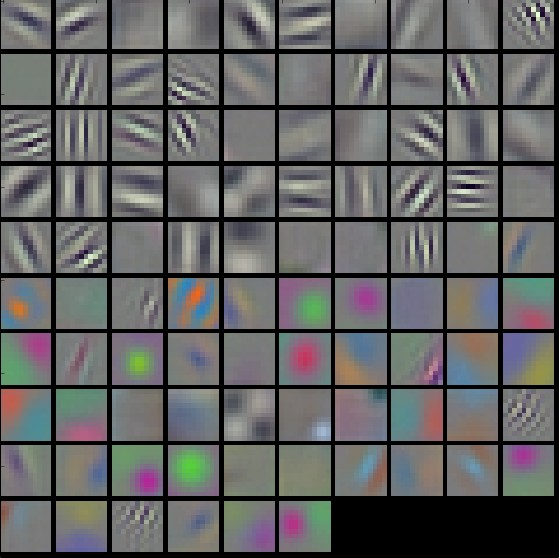
\includegraphics[scale=0.4]{images/sota/filt1.jpeg}
      % \caption{Visualization of the first convolution layer of a trained AlexNet. The weights are very nice and smooth, indicating nicely converged network. Note also the basic simple shape of filters. It easy to imagine that those same filters will be useful in other computer vision or image related tasks.}
      \caption[Convolution Neural Networks filters shape]{Visualization of the first convolution layer of a trained AlexNet. Note the basic shape of filters that resemble to Gabor filters widely used in image processing for decades \citep{fogel1989gabor,jain1991unsupervised}. It is possible to see that those same filters will be useful in other computer vision or image-related tasks.}
      \label{fig:AlexNet_filters}
    \end{figure}

    \par It is interesting to note that those filters can be also seen as a representation for the skills we want to extract. In our case, we will need to combine both deep convolution network with a recurrent neural network (like in \citep{s16010115,pinheiro2014recurrent,huang2016deep}).


    \paragraph{Sentiment Classification}
     \citep{glorot2011domain} discusses a deep learning approach for transfer learning for sentiment classification, by using stacked de-noising auto-encoders \citep{vincent2008extracting} to correct the marginal distribution between the source and the target domain, by learning latent variables/features common between the two data sources in two steps:
    \begin{itemize}
        \item First, train an auto-encoder on the unlabeled data from the source and the target. This will produce latent variables that will make $P(X_S)$ closer to $P(X_T)$.
        \item Use those latent features to train a classifier on the labeled source data.
    \end{itemize}
    \par Experiments are done on 12 different sources and target domain pairs. The data used reviews for different products (4 different products). The performance metric used in this case is the classification error rate when using a classifier trained on the source task only, minus the classification error rate of a classifier trained on the target task only. A SVM classifier trained on the source domain is used as a baseline, and a comparison with other transfer methods \citep{blitzer2006domain,li2008multi,pan2010cross}. All these methods performs better than the baseline, and \citep{glorot2011domain} peforms better than all of them.

    \paragraph{Underwater Acoustics}
     \citep{malfante2018use} compares the use of deep transfer learning to manual features \citep{malfante2016automatic,malfante2018machine}, in order to recognize the sounds of fish underwater. Interestingly, the deep learning models are trained on ImageNet \citep{imagenet_cvpr09} dataset (which is completely unrelated to acoustics), then used in order to extract features from the spectrogram of the underwater recordings. The assumption here is the the filters learned with deep learning are basic and generic enough, to be used in other domains, thus, deep learning can provide a natural correction for $P(X_S)$, to make it close to $P(X_T)$. Without any finetuning, the deep learning achieves quite a high perfomance, although less than the state of the art, suggesting that a further investment in this direction is worth the time.

    \paragraph{Speech modeling}
    \citep{xu2014cross} studies the idea of transfering the speech knowledge learned from one language pair to another using deep neural networks. In particular, the study the transfer between Mandarin and English (in both ways). Their hypothesis is that when modeling the speech in a language, there is a part in the model that is language independent. Their work was to find this part, and use it to bootstrap the learning of a new language (in case of neural networks, this can be rephrased as trying to find the good part in the neural network that is language independent).

    The compare to a deep learning model trained on the target task only, and compare the different the usage of different layers of a deep neural network trained on the source task (in order to determine the best part, or the language independent part). They report multiple performance metrics: segmental SNR (SSNR), log-spectral distortion (LSD), and perceptual evaluation of speech quality (PESQ). They find that, given insufficient data on the target task (which is one of the motivations to perform transfer learning), this transfer scheme works better than the baseline.

    \paragraph{Image classification}
    \citep{oquab2014learning} investigated the usage of a convolution neural network (CNN) trained on ImageNet \citep{imagenet_cvpr09} (where the object of interest is centered in the image), to extract low-level and mid-level features, that can transfer well to more complex dataset, PASCAL VOC \citep{everingham2010pascal} (where there are several objects of interest in the image), and is smaller than ImageNet. They use the \textit{average percision} as their peformance metric, and they show that the transfer is better than training a model from scratch on this target dataset.

    \paragraph{Styles of speech synthesis}
    \citep{wang2018style} discusses the problem of transfering the styles between different speakers, in the task of speech synthesis. Traditionally, the oucome of speech synthesis systems is the same style. One of the challenges is to capture the richness of style of different speakers on some training data, and transfer this style to new text. In their work, they propose an embedding approach called \textit{Global Style Tokens}, in order to extract the styles from the different speakers during the training phase. They then show that they can use these tokens as extra information to the speech synthesis system, to bias/affect the style of the outcome.
    They compare this to a baseline model, called \textit{TACOTRON} \citep{wang2017tacotron}, without these GST addition. They use \textit{Mean Opinion Score} (MOS) performance metric -- a subjective metric to assess the quality of experience experienced --. The report that transfer learning using GST outperforms the usage of the baseline model.

  % \subsection{Adversarial-based transfer learning}
  % \par Encouraged by the recent advances in generative adversarial networks (GANs) \citep{goodfellow2014generative}, a new line work is trying to utilise this tool to achieve transfer learning, on the assumption that a good representation (suitable for transfer) should be general enough that it does not discriminate between the source and the target domains, yet discriminative enough to learn the required tasks on either domains.
  %
  % \subsection{Negative transfer}
  % \par A concern that arises in transfer learning is what is called \textit{negative transfer}, where the knowledge learned from one task leads to no improvement on the target task, or reduction in the quality of learning for that task. This can happen for multiple reasons \citep{rosenstein2005transfer}:
  % \begin{itemize}
  %     \item The source task is not sufficiently related to the target task, thus, in the best case scenario, no useful knowledge can be transferred.
  %     \item The transfer method is not able to exploit the similarities between the source and the target task
  % \end{itemize}
  % In \citep{rosenstein2005transfer}, the authors studied this problem, and provided examples for negative transfer.
  % Within the framework of \textit{reinforcement learning}, some methods can estimate task similarity \citep{taylor2008transferring, torrey2010transfer}, though these methods do not provide any theoretical guarantees about their effectiveness. This, however, is an open area of investigation in the framework of \textit{supervised learning} \textbf{CAN'T FIND RESOURCES HERE}. The main thing here for us to be careful during the choice/design of the source and the target experiments, to ensure that a possible positive transfer learning can happen.

\section{Putting it all together}
  \par In the previous section, we explored the concept of transfer learning, with focus on network-based transfer, with multiple examples from the literature on this type of transfer. In the section, I will explain the work done during the PhD on transfer learning. The main challenge we had is how to capture and transfer the styles between different tasks. This proposes multiple questions:
  \begin{itemize}
    \item Which framework/methodology of transfer we should use?
    \item How to assess the quality of transfer?
  \end{itemize}

  \par In this part, we study these questions on both \textit{IRONOFF} and \textit{QuickDraw!}. Our experimental setup is inspired by the work done in \citep{8686063}. We use a slightly different experimental protocol between the two datasets however. I will discuss the reasoning behind this, and will argue that both setups are good enough to address our questions concerning the transfer of styles.

  \par Concerning the performance metrics, we decided to use multiple metrics to determine the effect of transfer learning, and compare it to the baseline (no transfer). While the usage of a single metric offers more convenience for decision making (i.e., which model to choose), our goal is have a better understanding for the transfer of style. To achieve this, we would like to shade light on the outcome from different angles, by using multiple metrics. We first evaluate the quality of the model in prediction by looking at the loglikelihood (crossentropy) on the test data\endnote{Based on experience, the crossentropy matters when it comes to generation. A difference of around 0.1 in crossentropy between two models gives different generation quality.}. We then evaluate the quality of generation using our previously proposed metrics (the BLEU score and EOS analysis). We compare perform the generated strokes count, and include it in the comparison.

  \par One of the things we changed from the previous work is that, when analysing \textit{end of sequence}, instead of using Pearson Coefficient, we use Krippendorff-Alpha \citep{krippendorff2011computing}. The reason for this is that it offers a smoother transition between what is good and bad. In Pearson coefficient, if there is a mismatch between the generation and ground truth, it will not matter how big is the mistake (the distance between the generated and the ground truth). With Krippendorff-alpha, we can consider the distance in the analysis, thus providing a softer and more realistic estimation for the correlation.

  \par Another aspect we consider in our analysis is \textit{strokes} the model is generating. In the previous work, we did not model the strokes, in order to simplify the system and the analysis. Now that we are confident about our approach, we added the strokes to our model. Strokes are more complex to model, because they the stroke signals are more sparse. A good stroke generation is an indication that the model can perform hard discrete decisions in order to generate the whole shape. We use Krippendorff coefficients as well to report and analyze the strokes. We also consider the confusion matrices for the generated strokes versus the ground truth ones, in order to shade more light on the behavior of the model.

  \par One important choice to make is to decide the amount of data to be used in the target task. Normally, the whole point from transfer learning is to address the insufficient data available for the target task. However, since we do not have a particular scenario to solve (we are mainly interested in that 'what if this happens' question), there is no clear criteria to decide the amount of data. If we select very few points, we may be biased towards giving transfer learning an advantage, while also sacrificing having generally bad results (even if transfer learning proved to be better than baseline on our performance metrics). It is important that the overall behavior of the system is acceptable (generating shapes with acceptable quality). To get around this design problem, we decided to use the entire data available to the target task, thus, testing the 'worst case scenario' for transfer learning (where the baseline has plenty of data, and it is used to train the whole model, compared to training only half the model in case of transfer learning). This will be the case for both \textit{IRONOFF} and \textit{QuickDraw!} datasets.

  \subsection{IRONOFF}
    \par In case of handwriting letters, we define the task by the higher category it belongs to. So we have 3 tasks: uppercase, lowercase and digits\endnote{I do not see a problem of working on the lower categories (A, a, B, b, ...., 7, 8, 9). However, it would have consumed a lot of computational time test on all possible combinations of source/target tasks.}.
    \par We explore the idea of transfer learning on all possible combinations of tasks:
    \begin{itemize}
      \item From uppercase and lowercase to digits,
      \item from uppercase and digits to lowercase,
      \item and from lowercase and digits to uppercase.
    \end{itemize}

    \subsubsection{Experimental setup}
      \par Figure \ref{fig:ironoff_protocol} details the protocol we used for this experiment. For each source/target task combination, we first perform hyperparameter search for the network for both the source and the target tasks. The best performing hyperparameters gives use the source and the target models. Using these models:
      \begin{itemize}
        \item We use the source model to extract the encoder module (aka, the style extraction module). We then add it to a new model, freeze it (it will not be part of training), and train the new model on the target task. We also search for the best hyperparameters for this new model. We call this model the 'transfer model'. We retrain this transfer model 5 times with different random weights each time, and report the stats on the crossentropy of the test data for these repetitions.
        \item We retrain the target model 5 time as well.
        \item Then, we use the best performing transfer and targets models for generating the target tasks, and report the stats of the different generation metrics.
      \end{itemize}
      \par We use 10\% of the data for testing, another 10\% for validation, and the rest is our training set.

    \begin{sidewaysfigure}[htbp]
      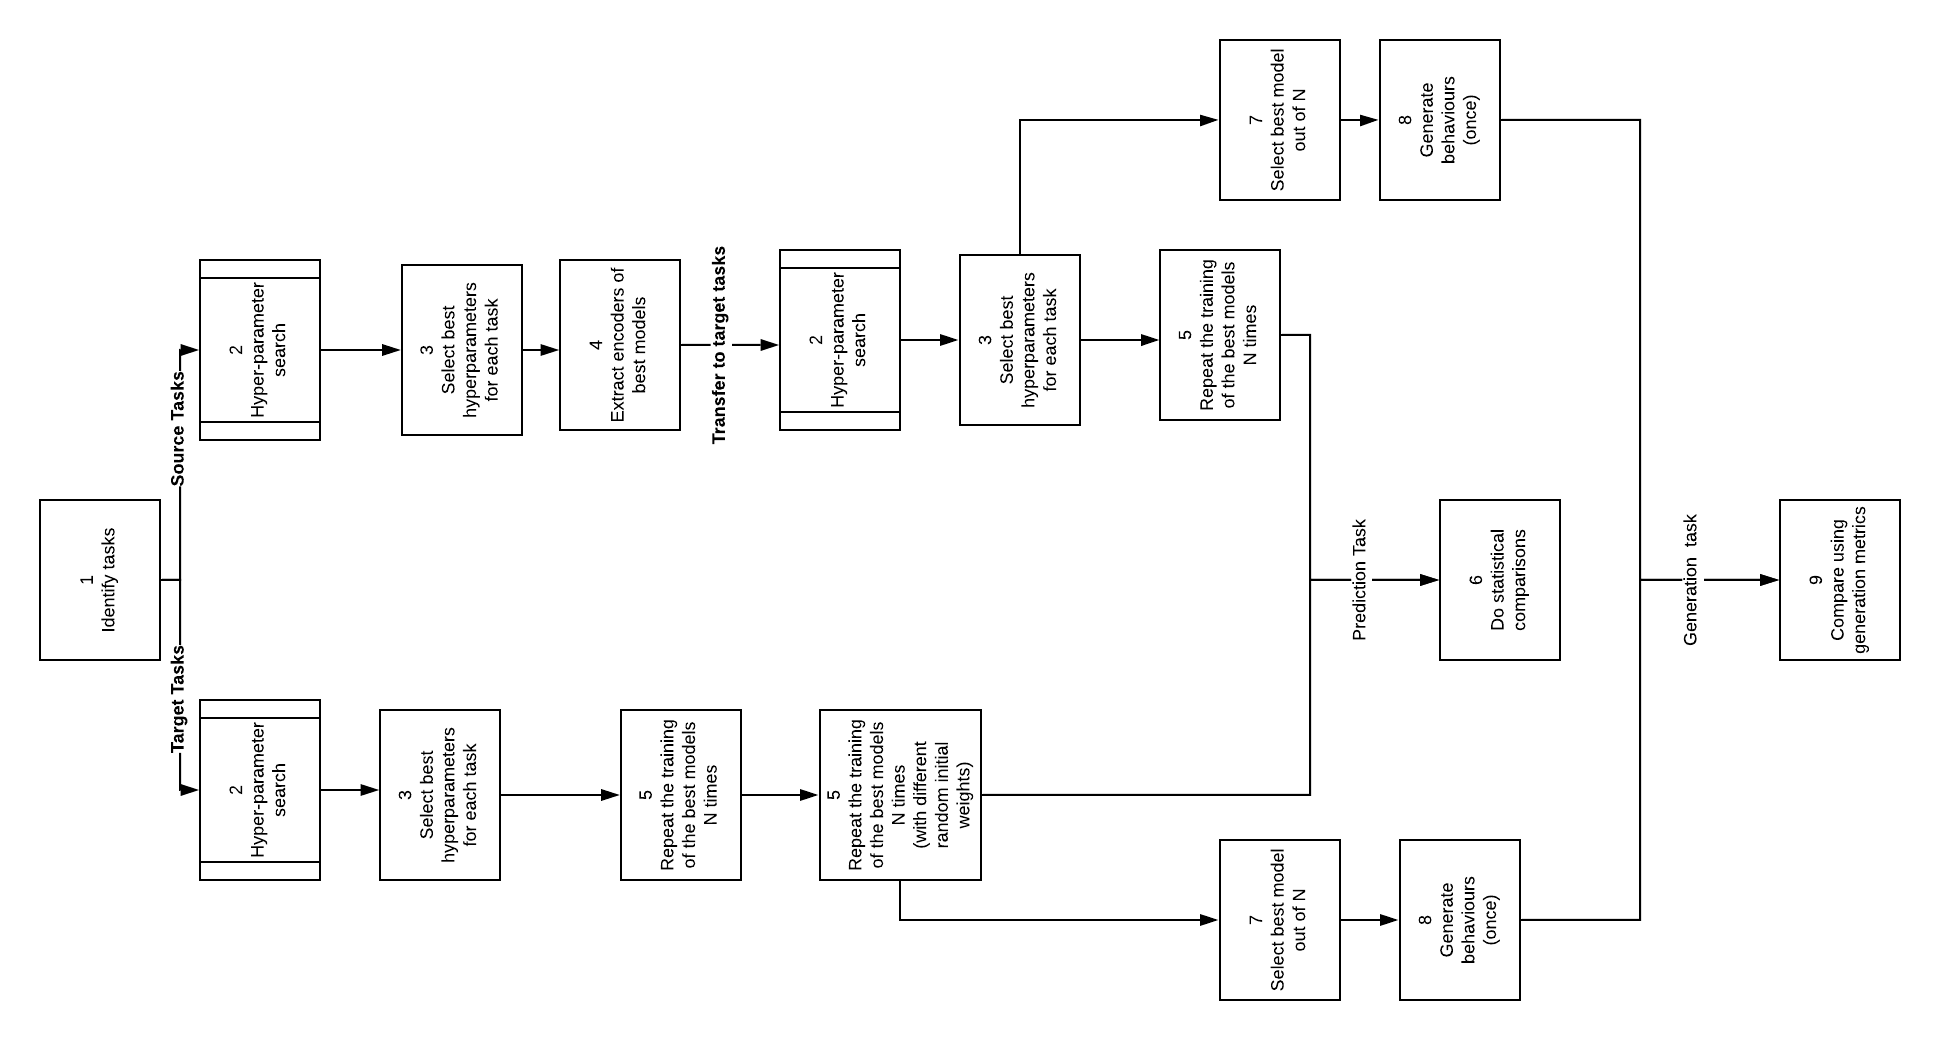
\includegraphics[scale=0.3]{images/sota/ironoff_results/IRONOFF_transfer_learning_flow.png}
      \caption{Flow chart explaining the experiment protocol used in \textit{IRONOFF} dataset.}
      \label{fig:ironoff_protocol}
    \end{sidewaysfigure}

    \subsubsection{Results}
    \paragraph{Loglikelihood of prediction}
      In the prediction mode, the model is tested in a similar manner to the way it was trained: it is given the input from the ground truth, representing the current timestep, and asked to predict the next timestep. This tells us about the quality of the training procedure from one side, and shade light on the confidence of the model in predicting the next timestep.

      The result of 5 times repetitions, for all the different combinations of source/target tasks, are mentioned in figure \ref{fig:ironoff_crossentropy}. We can see that the transfer learning always gives a significant advantage over baseline models.
      \begin{sidewaysfigure}
        \centering
          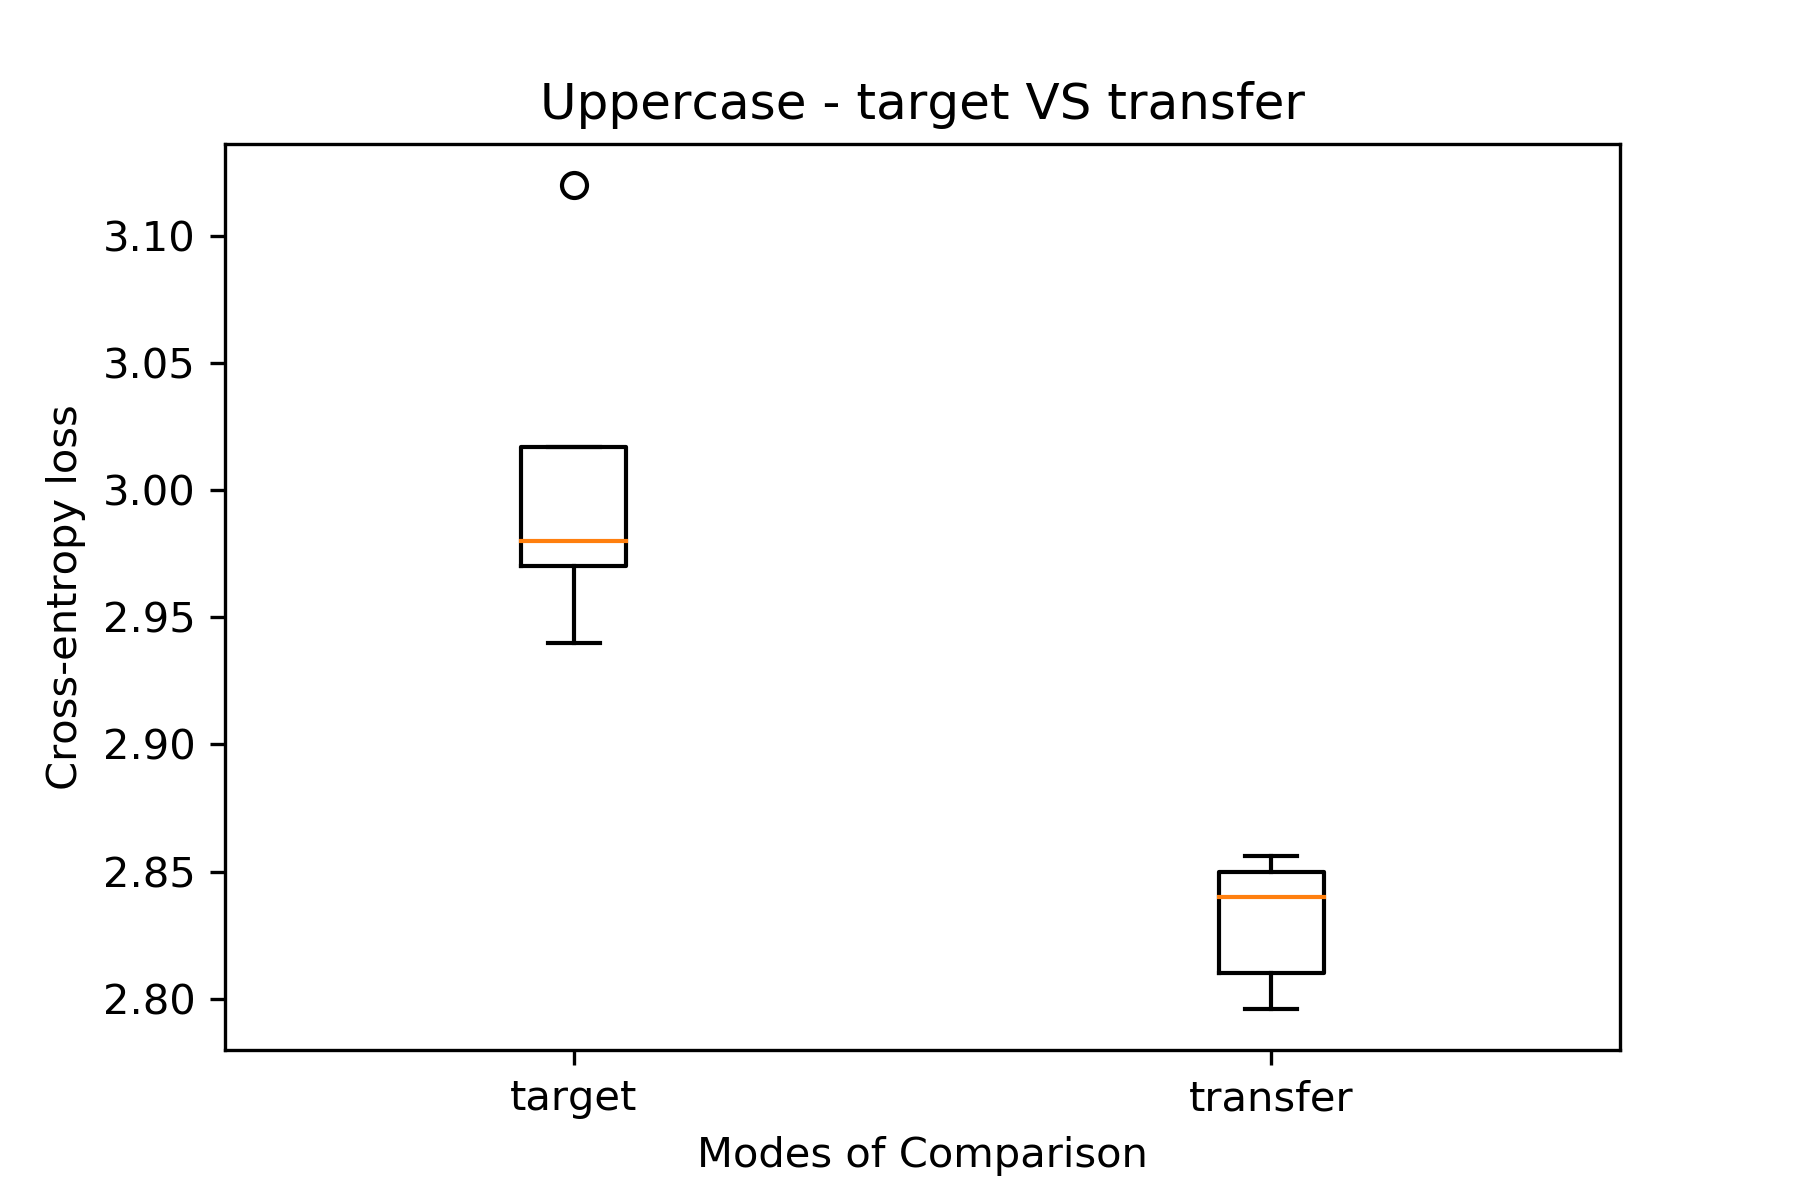
\includegraphics[width=0.48\textwidth]{images/sota/ironoff_results/uppercase.png}\quad
          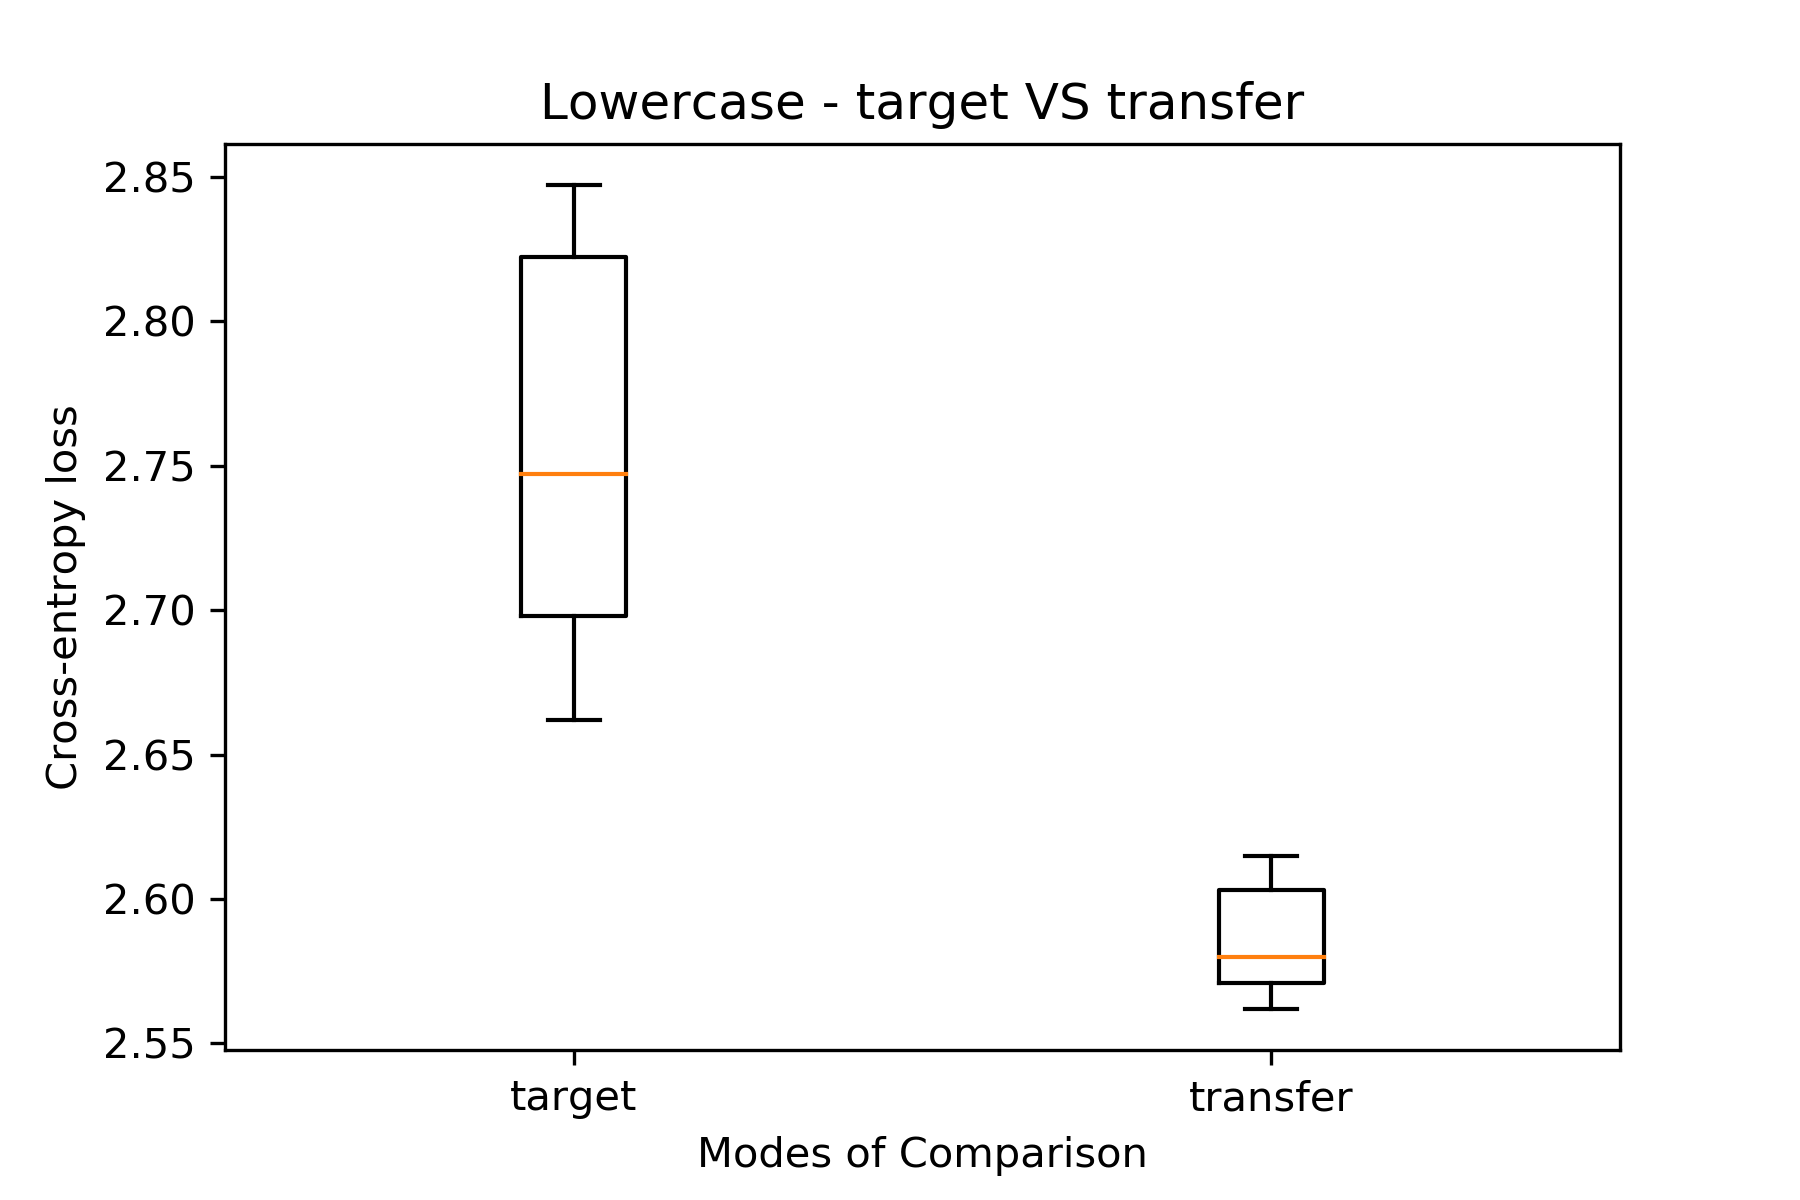
\includegraphics[width=0.48\textwidth]{images/sota/ironoff_results/lowercase.png}\quad
          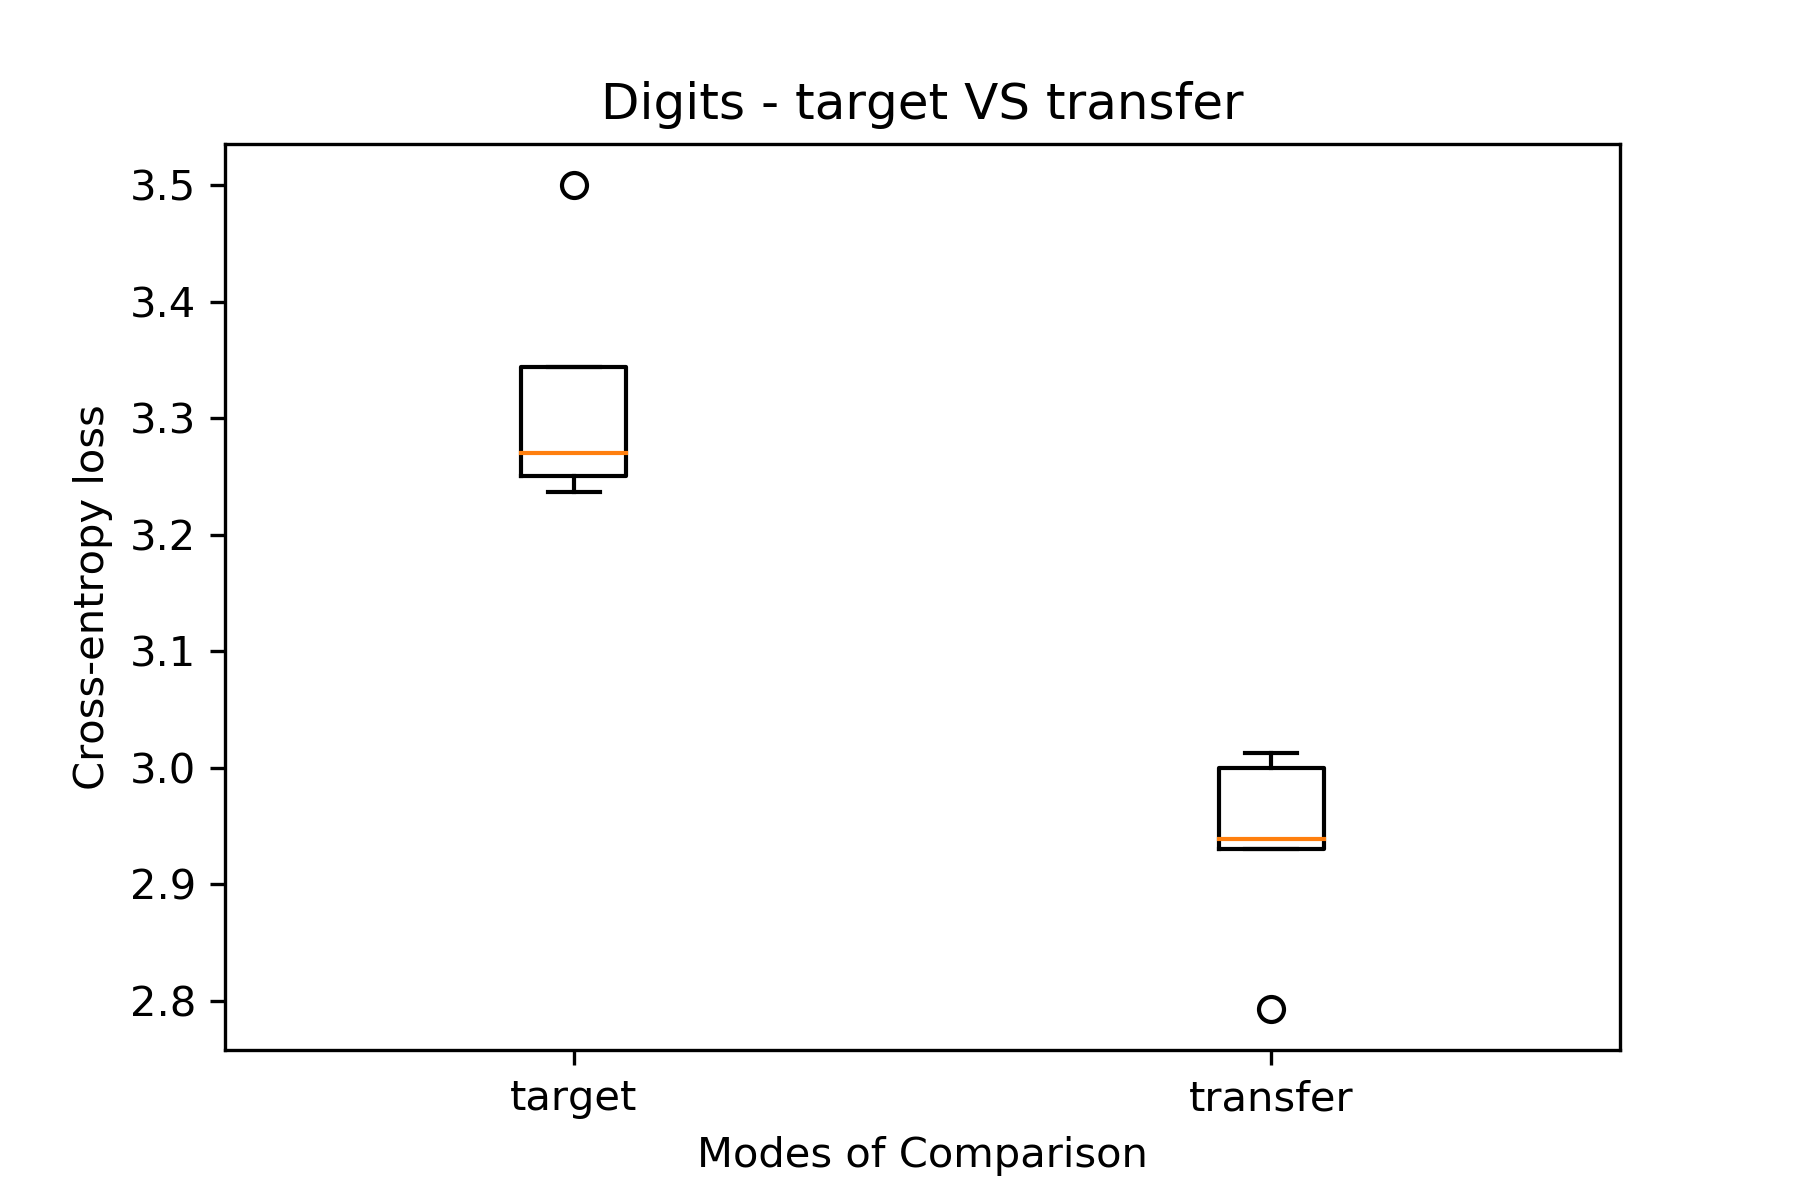
\includegraphics[width=0.48\textwidth]{images/sota/ironoff_results/digits.png}
        \caption{IRONOFF - crossentropy of prediction of test dataset for different combinations of source/target tasks, with 5 repetitions. We can see that, in all possible source/target task combinations, the transfer learning gives better advantage than just learning from scratch on the target task.}
        \label{fig:ironoff_crossentropy}
      \end{sidewaysfigure}

    \paragraph{BLEU score}
      Now we go to the generation part, our main concern in this thesis. As discussed earlier, we use BLEU score to assess the quality of matching segments between the generated and the ground truth letters, in a gradual manner (i.e., we increase the size of the segments to match gradually). Table \ref{table:bleu_score_ironoff_transfer} summarizes the numbers. We see that transfer learning always performs better than the baseline.
    \paragraph{End-of-Sequence analysis}
    One aspect to measure the quality of the generation, that we identified previously, is to analyse how the model anticipate the end of the sequence generation. Table \ref{table:ironoff_eos_transfer} shows the results of the Krippendorff coefficients for the different modes. In general, the different modes are performing quite well. It can be seen that transfer learning is actually performing better than the baseline models, adding another indication to the benefit of using transfer learning.

    \paragraph{Strokes analysis}
    As mentioned earlier in this section, we started to consider the the strokes in this part of our work. Table \ref{table:ironoff_strokes_transfer} shows the strokes results of the Krippendorff coefficients for the different modes. With the exception for the uppercase letters, transfer learning performs better than baseline models. For the uppercase, this could be due extra complixty these letters presents (see figure \ref{fig:ironoff_strokes}, where it can be found that uppercase letters are usually the ones with higher number of strokes). A fine tuning for the style extraction module is the next logical step to perform here, to make it adapt to complexity of the this task. We also consider the confusion matrix for the generated strokes in comparison with the ground truth, figure \ref{fig:ironoff_strokes_cnf}. We can see that it is consistant with the Krippendorff results, where transfer learning outperforms the baselines. In the uppercase letters however, it is notable that the transfer learning performs better on the single stroke, while the baseline performs better on the 2 and 3 strokes.

      \begin{table}[!htbp]
        \centering
        \begin{tabular}{|l||c|c|c||c|c|c|}
          \hline
          \multicolumn{1}{|c||}{Aspect/Feature} & \multicolumn{3}{c||}{ Speed } & \multicolumn{3}{c|}{ Freeman }   \\ \hline
          Model / B-score      & B-1  & B-2  & B-3           & B-1  & B-2   & B-3              \\ \hline
          Uppercase-baseline &   66.1 & 46.3 & 27.2 & 62.8 & 49.4 & 37.1 \\\hline
          Uppercase-transfer &   68.3 & 47.8 & 28.3 & 65.47 & 51.8 & 39.0 \\\hline

          Lowercase-baseline &   73.13 & 69.7 & 55.9 & 54.82 & 37.2 & 40.9 \\\hline
          Lowercase-transfer &   75.54 & 71.17 & 58.0 & 56.0 & 39.4 & 41.9 \\\hline

          Digits-baseline &    68.7 & 65.23 & 49.12 & 49.57 & 29.28 & 34.6  \\\hline
          Digits-transfer &    71.47 & 70.72 & 51.2 & 55.9 & 31.36 & 41.7 \\\hline

        \end{tabular}
        \caption{IRONOFF: BLEU score results on the generated letters, for the baseline models (trained on the target task only), and the transfer models (the encoder -- style extractor -- is trained on the source task, while the decoder is trained on the target task). The results show an advantage in using transfer learning.}
        \label{table:bleu_score_ironoff_transfer}
      \end{table}

      \begin{table}[!htbp]
        \centering
        \begin{tabular}{|l|c|c|}
        \hline
        Models & Krippendorff coefficient\\ \hline
        Uppercase-baseline & 0.951 \\ \hline
        Uppercase-transfer &  0.97\\ \hline
        Lowercase-baseline & 0.957 \\ \hline
        Lowercase-transfer & 0.996 \\ \hline
        Digits-baseline & 0.916 \\ \hline
        Digits-transfer & 0.985 \\ \hline
        \end{tabular}
        \caption{IRONOFF: Krippendorff correlation coefficients for the End-Of-Sequence (EoS) distributions between the transfer and baseline, for all tasks.}
        \label{table:ironoff_eos_transfer}
      \end{table}

      \begin{table}[!htbp]
        \centering
        \begin{tabular}{|l|c|c|}
        \hline
        Models & Krippendorff coefficient\\ \hline
        Uppercase-baseline & 0.379 \\ \hline
        Uppercase-transfer & 0.247 \\ \hline
        Lowercase-baseline & 0.558 \\ \hline
        Lowercase-transfer & 0.65 \\ \hline
        Digits-baseline & 0.398 \\ \hline
        Digits-transfer & 0.713 \\ \hline
        \end{tabular}
        \caption{IRONOFF: Krippendorff correlation coefficients for the strokes distributions between the transfer and baseline, for all tasks.}
        \label{table:ironoff_strokes_transfer}
      \end{table}

      % Strokes conf matrix
      \begin{figure}[!htbp]
        \centering
        \begin{subfigure}[tb]{0.45\textwidth}
            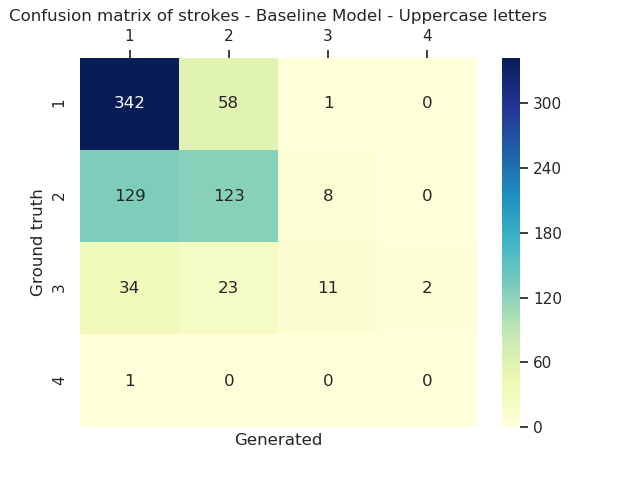
\includegraphics[width=\textwidth]{images/sota/ironoff_results/True_upper_strokes_heatmap.png}
        \end{subfigure}
        ~
        \begin{subfigure}[tb]{0.45\textwidth}
            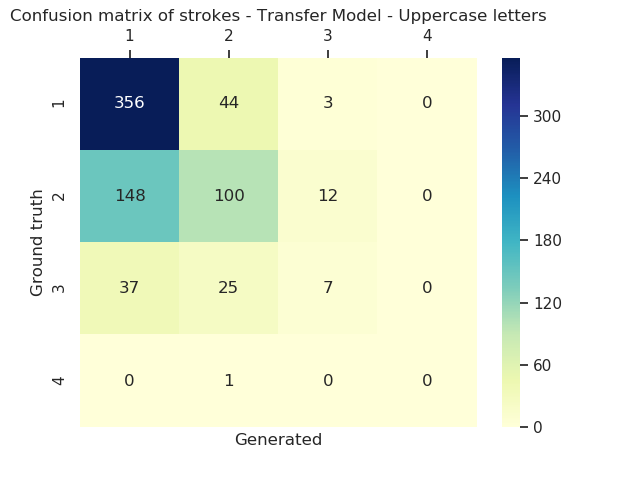
\includegraphics[width=\textwidth]{images/sota/ironoff_results/False_upper_strokes_heatmap.png}
        \end{subfigure}

        ~
        \begin{subfigure}[tb]{0.45\textwidth}
            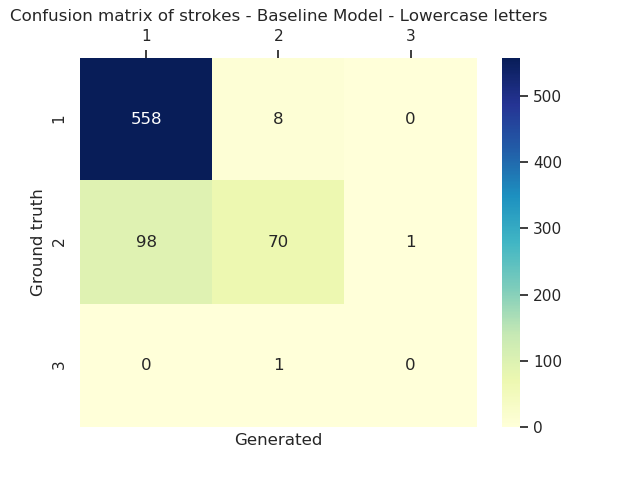
\includegraphics[width=\textwidth]{images/sota/ironoff_results/True_lower_strokes_heatmap.png}
        \end{subfigure}
        ~
        \begin{subfigure}[tb]{0.45\textwidth}
            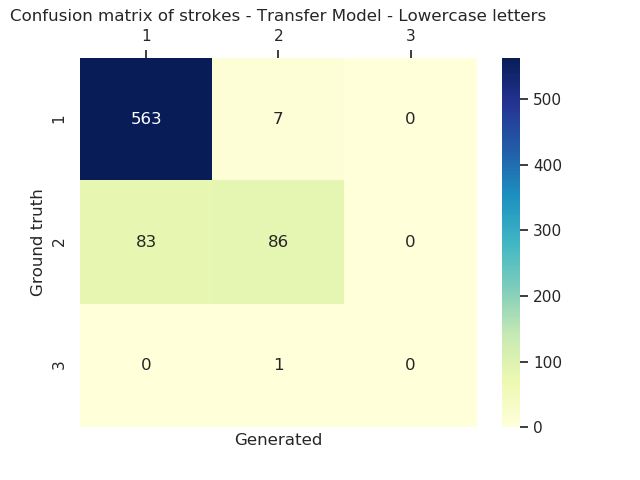
\includegraphics[width=\textwidth]{images/sota/ironoff_results/False_lower_strokes_heatmap.png}
        \end{subfigure}

        ~
        \begin{subfigure}[tb]{0.45\textwidth}
            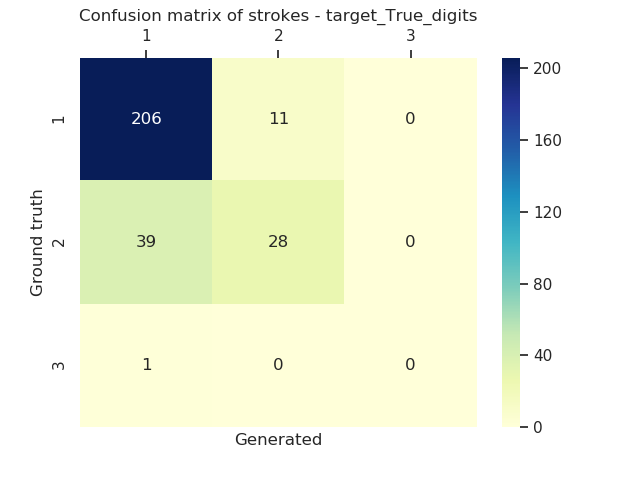
\includegraphics[width=\textwidth]{images/sota/ironoff_results/True_digits_strokes_heatmap.png}
        \end{subfigure}
        ~
        \begin{subfigure}[tb]{0.45\textwidth}
            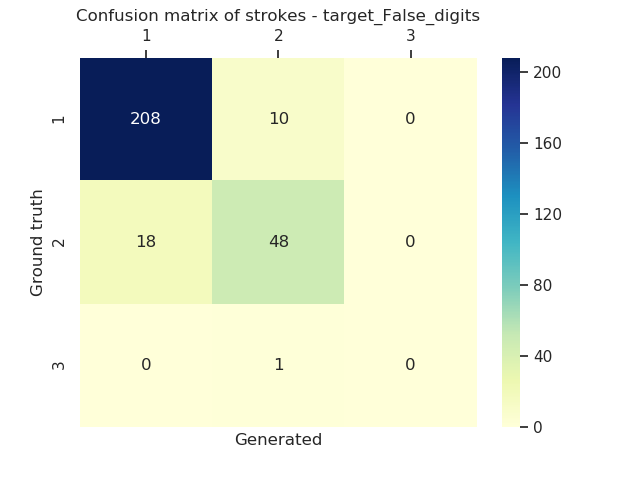
\includegraphics[width=\textwidth]{images/sota/ironoff_results/False_digits_strokes_heatmap.png}
        \end{subfigure}

        \caption{\textit{IRONOFF!}: Confusion matrix for strokes for both baseline and transfer modes, on the different tasks.}
        \label{fig:ironoff_strokes_cnf}

      \end{figure}

  \subsection{QuickDraw!}
    \par In case of sktech drawings, we define the task by the class it belongs to. So we have 5 tasks: circle, triangle, square, hexagon and octagon. We explore the idea of transfer learning on all possible combinations of tasks: in each combination, one task is removed (the target task), and the other task are considered source tasks.

    \subsubsection{Experimental setup}
    \par Due to the increase the number of tasks -- compared to \textit{IRONOFF} --, and using the same experiment setup proved to be too much compared to the computational budget available to us. We identify that one of the expensive bottlenecks in our work is the number of times we need to perform hyperparameter search. In order to get around this problem, we are using a simpler (and less powerful protocol), see figure \ref{fig:quickdraw_protocol}. We perform the hyperparameter search once in the beginning of the experiment, on the all the tasks combined, to find a good hyperparameter that is suitable to the domain of 'sketch drawing'. From there, we fix the hyperparameters for all the different steps in the experiment. The analysis steps are the same like in \textit{IRONOFF}.

    Another thing we noticed is that retraining the model 5 times only (like in \textit{IRONOFF}) only leads to unstable conclusions, thus make it hard to quantify the difference between the baseline and the transfer modes. We increased the number of models to 30 in this case, in order to have a more consistent trend.

    \begin{sidewaysfigure}[htbp]
      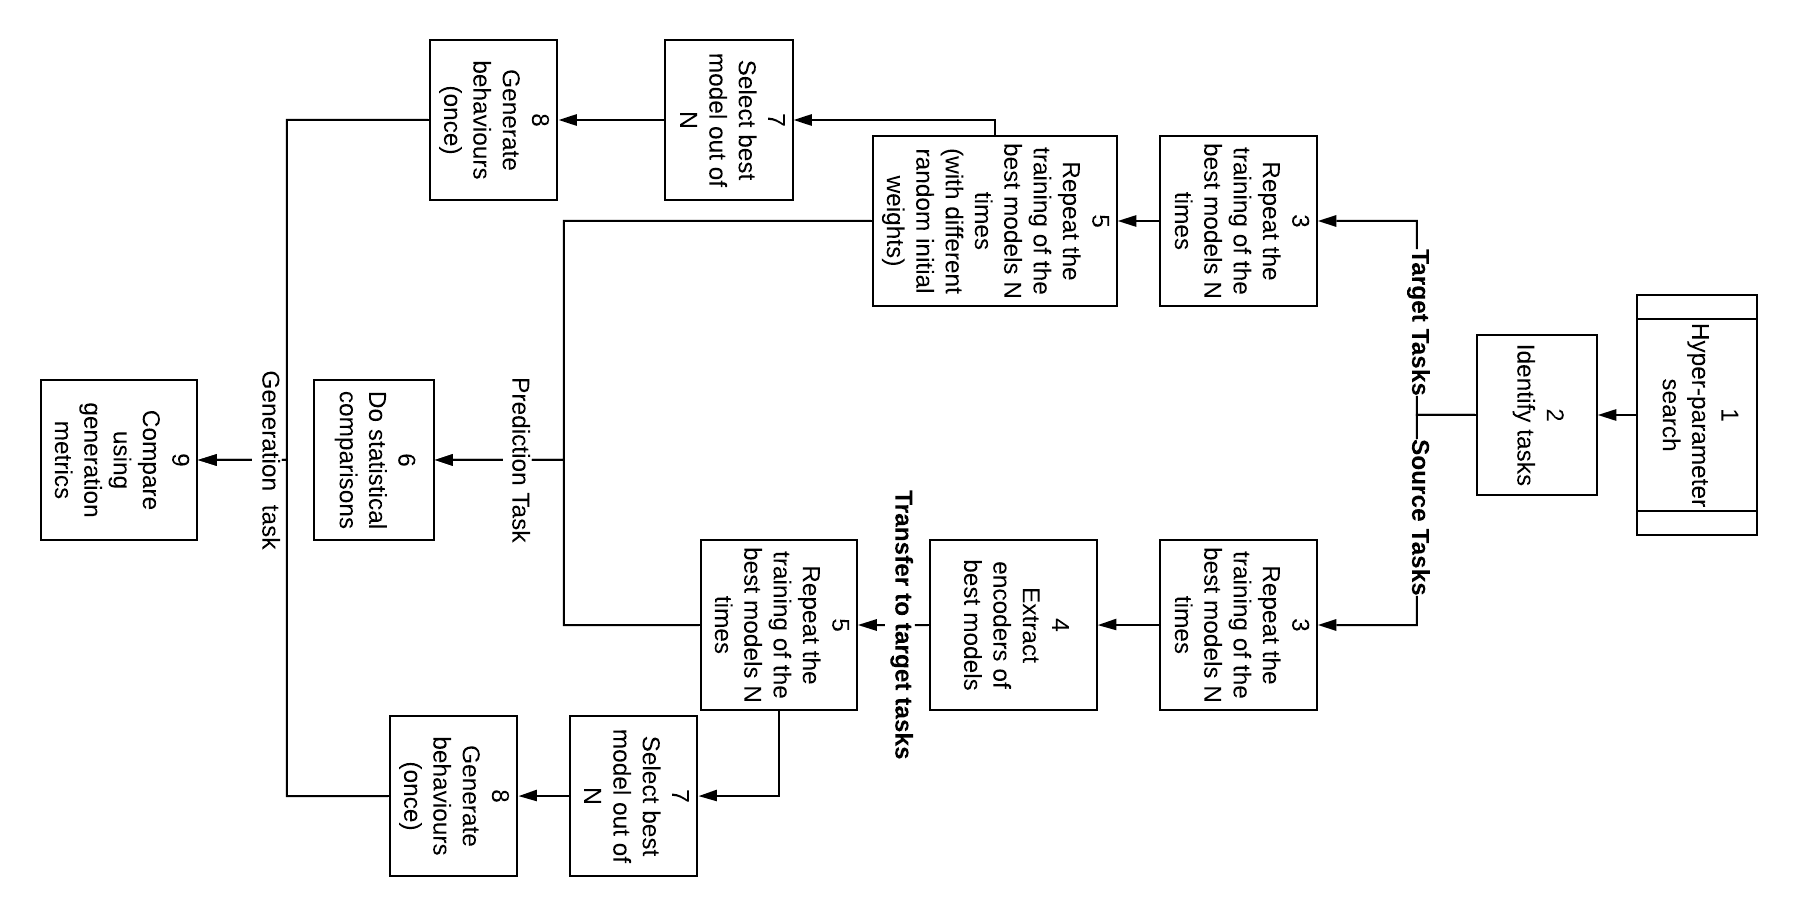
\includegraphics[scale=0.3]{images/sota/quickdraw_results/QuickDraw_transfer_learning_flow.png}
      \caption{Flow chart explaining the experiment protocol used in \textit{QuickDraw!} dataset.}
      \label{fig:quickdraw_protocol}
    \end{sidewaysfigure}

    \subsubsection{Results}
      \paragraph{Loglikelihood of prediction}
        The results can be seen in figure \ref{fig:quickdraw_crossentropy}. For all the combinations, there is a clear advantage for using transfer learning over the baseline model. The difference in all cases is statistically significant.
        \begin{sidewaysfigure}
          \centering
            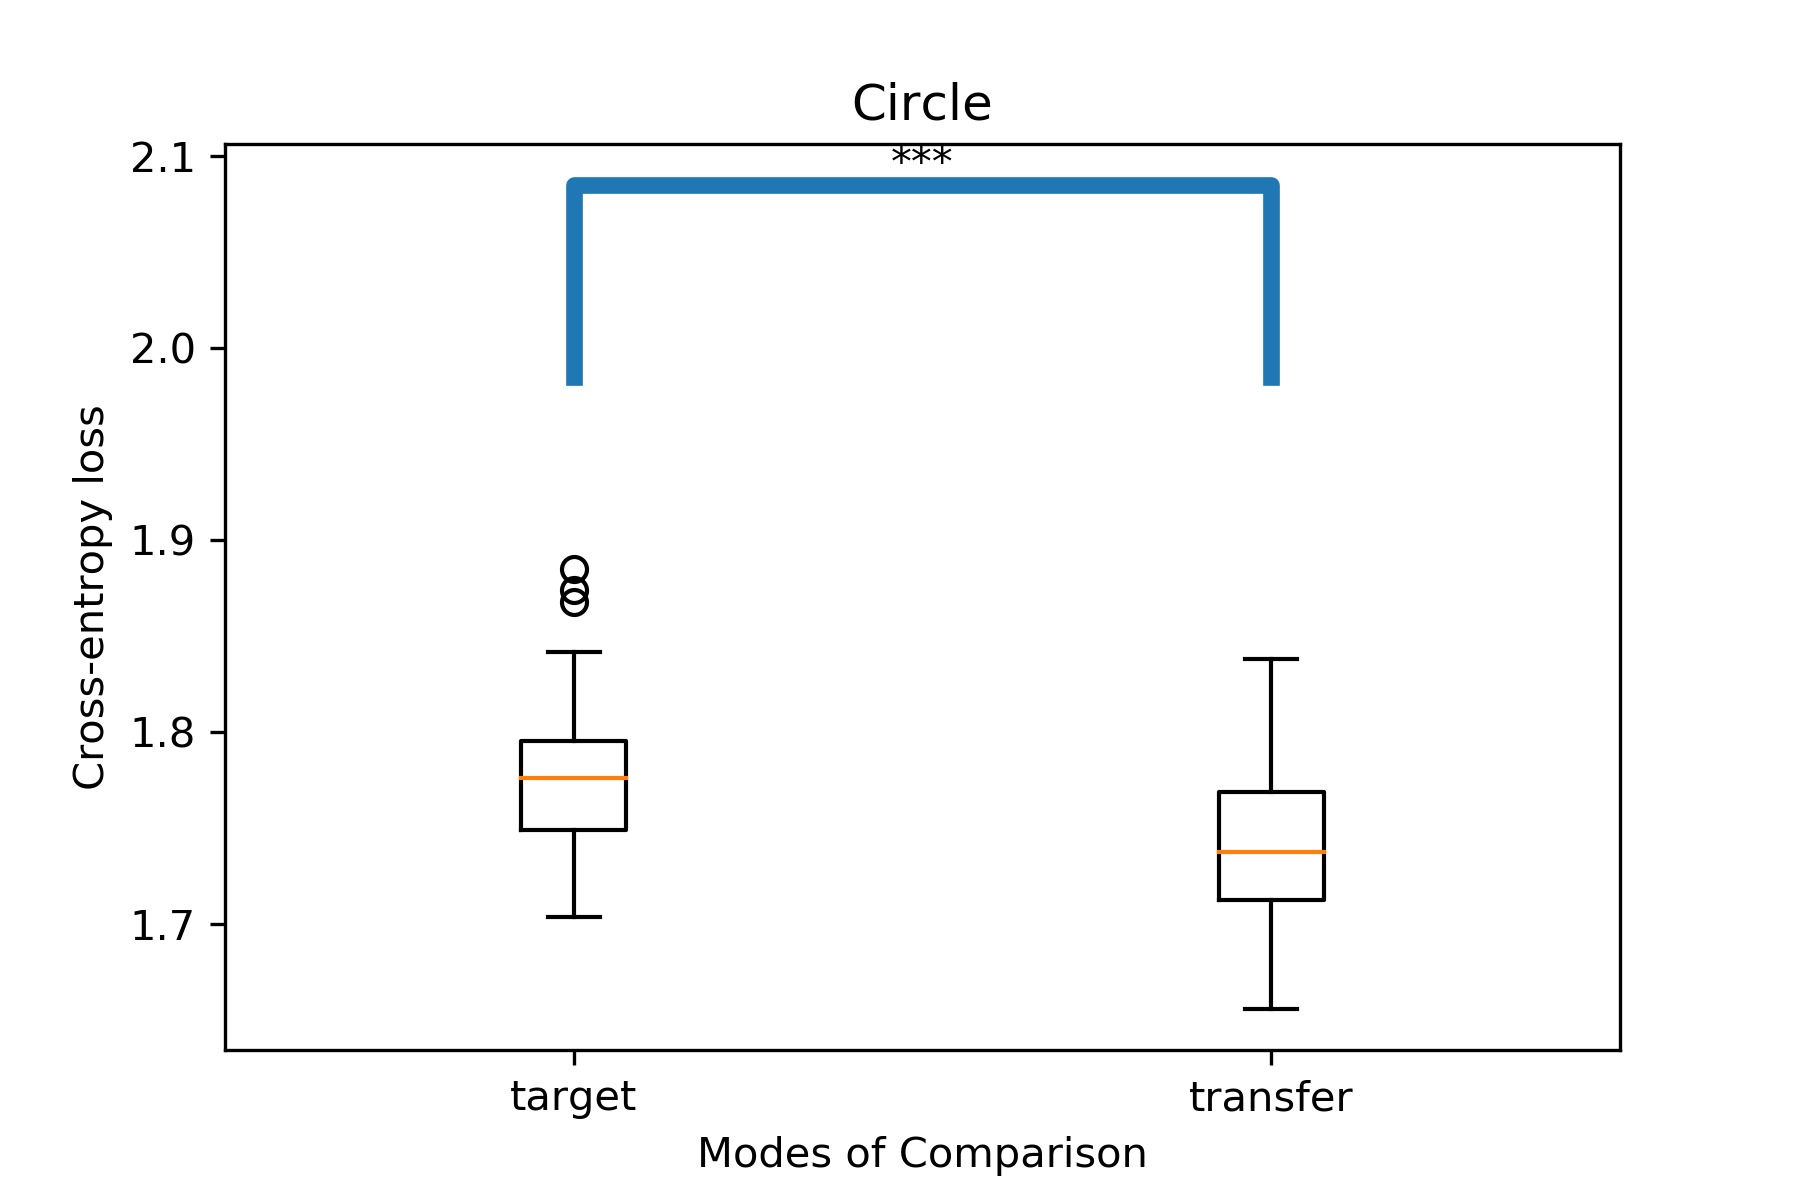
\includegraphics[width=0.31\textwidth]{images/sota/quickdraw_results/cir_ce.png}\quad
            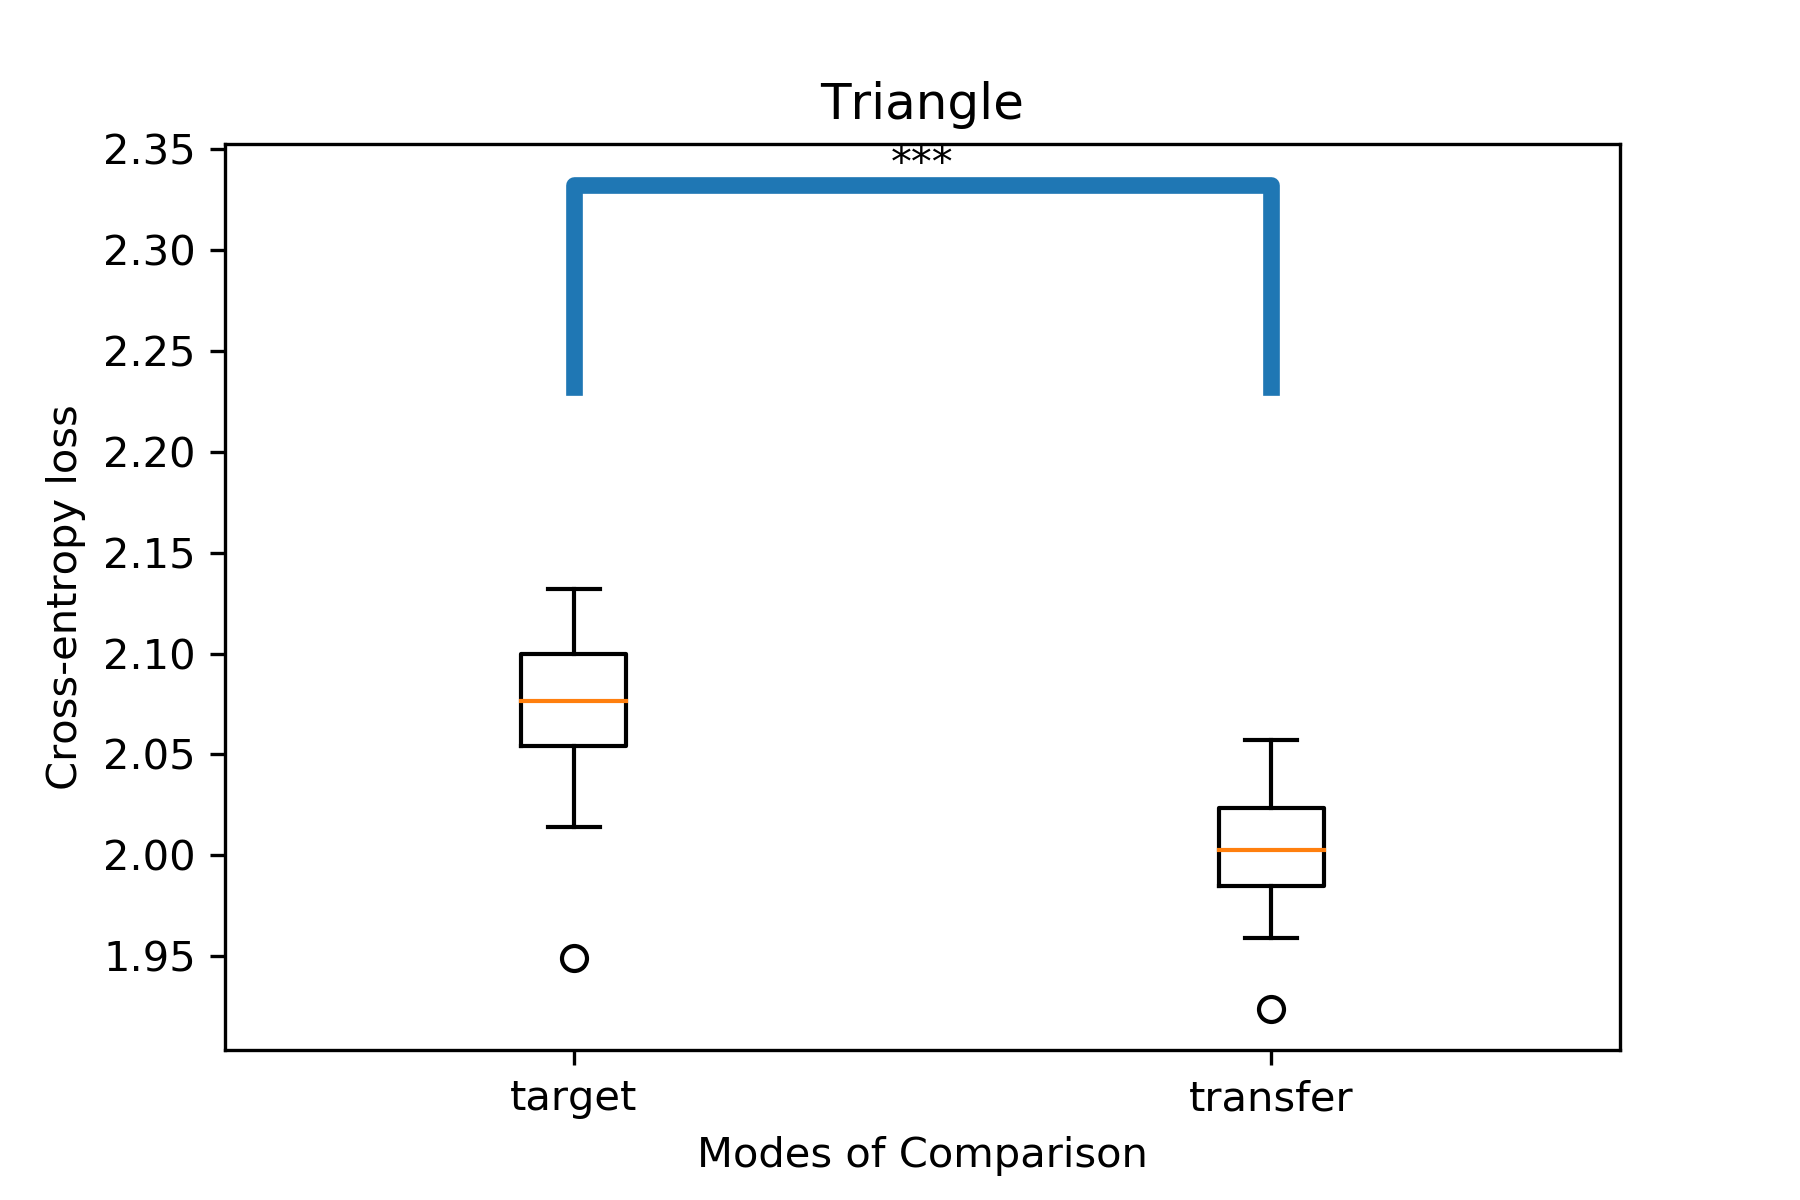
\includegraphics[width=0.31\textwidth]{images/sota/quickdraw_results/tri_ce.png}\quad
            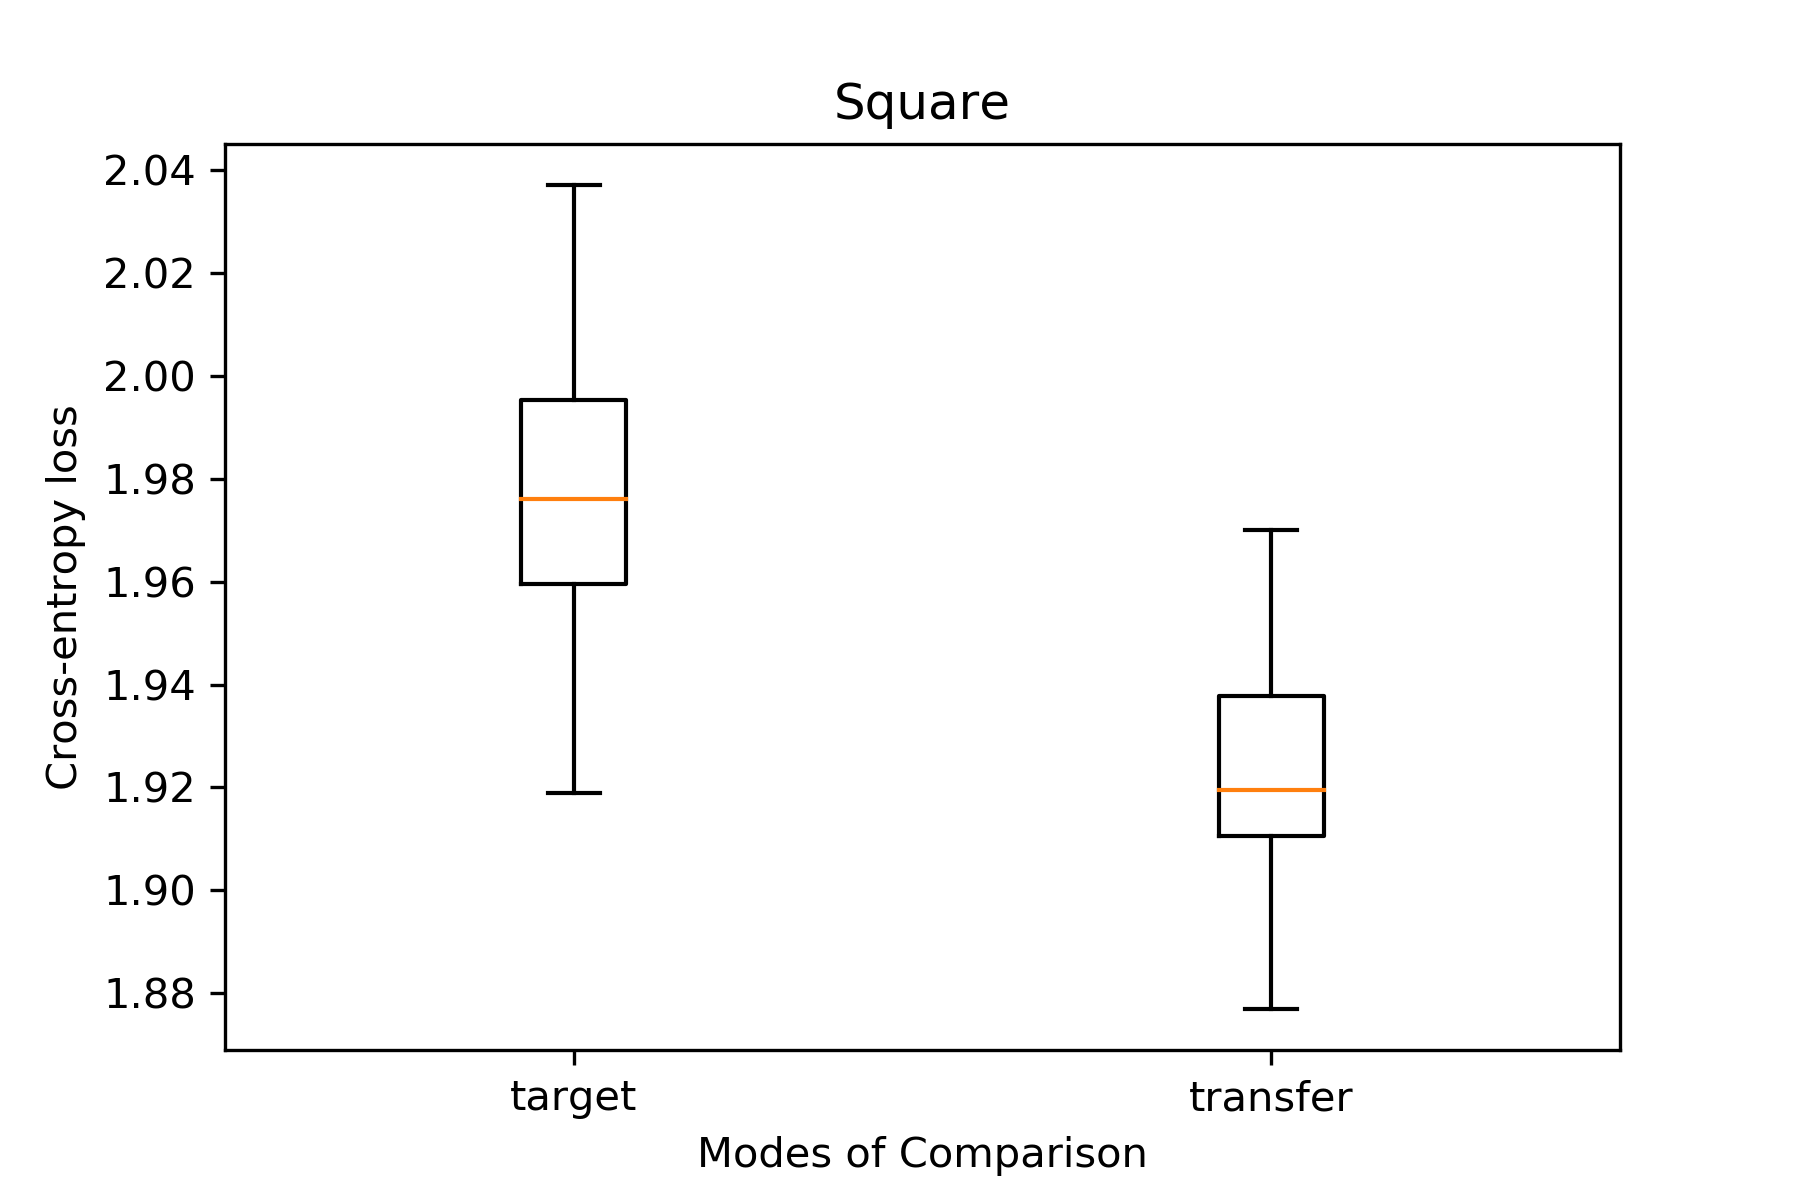
\includegraphics[width=0.31\textwidth]{images/sota/quickdraw_results/sq_ce.png}\quad
            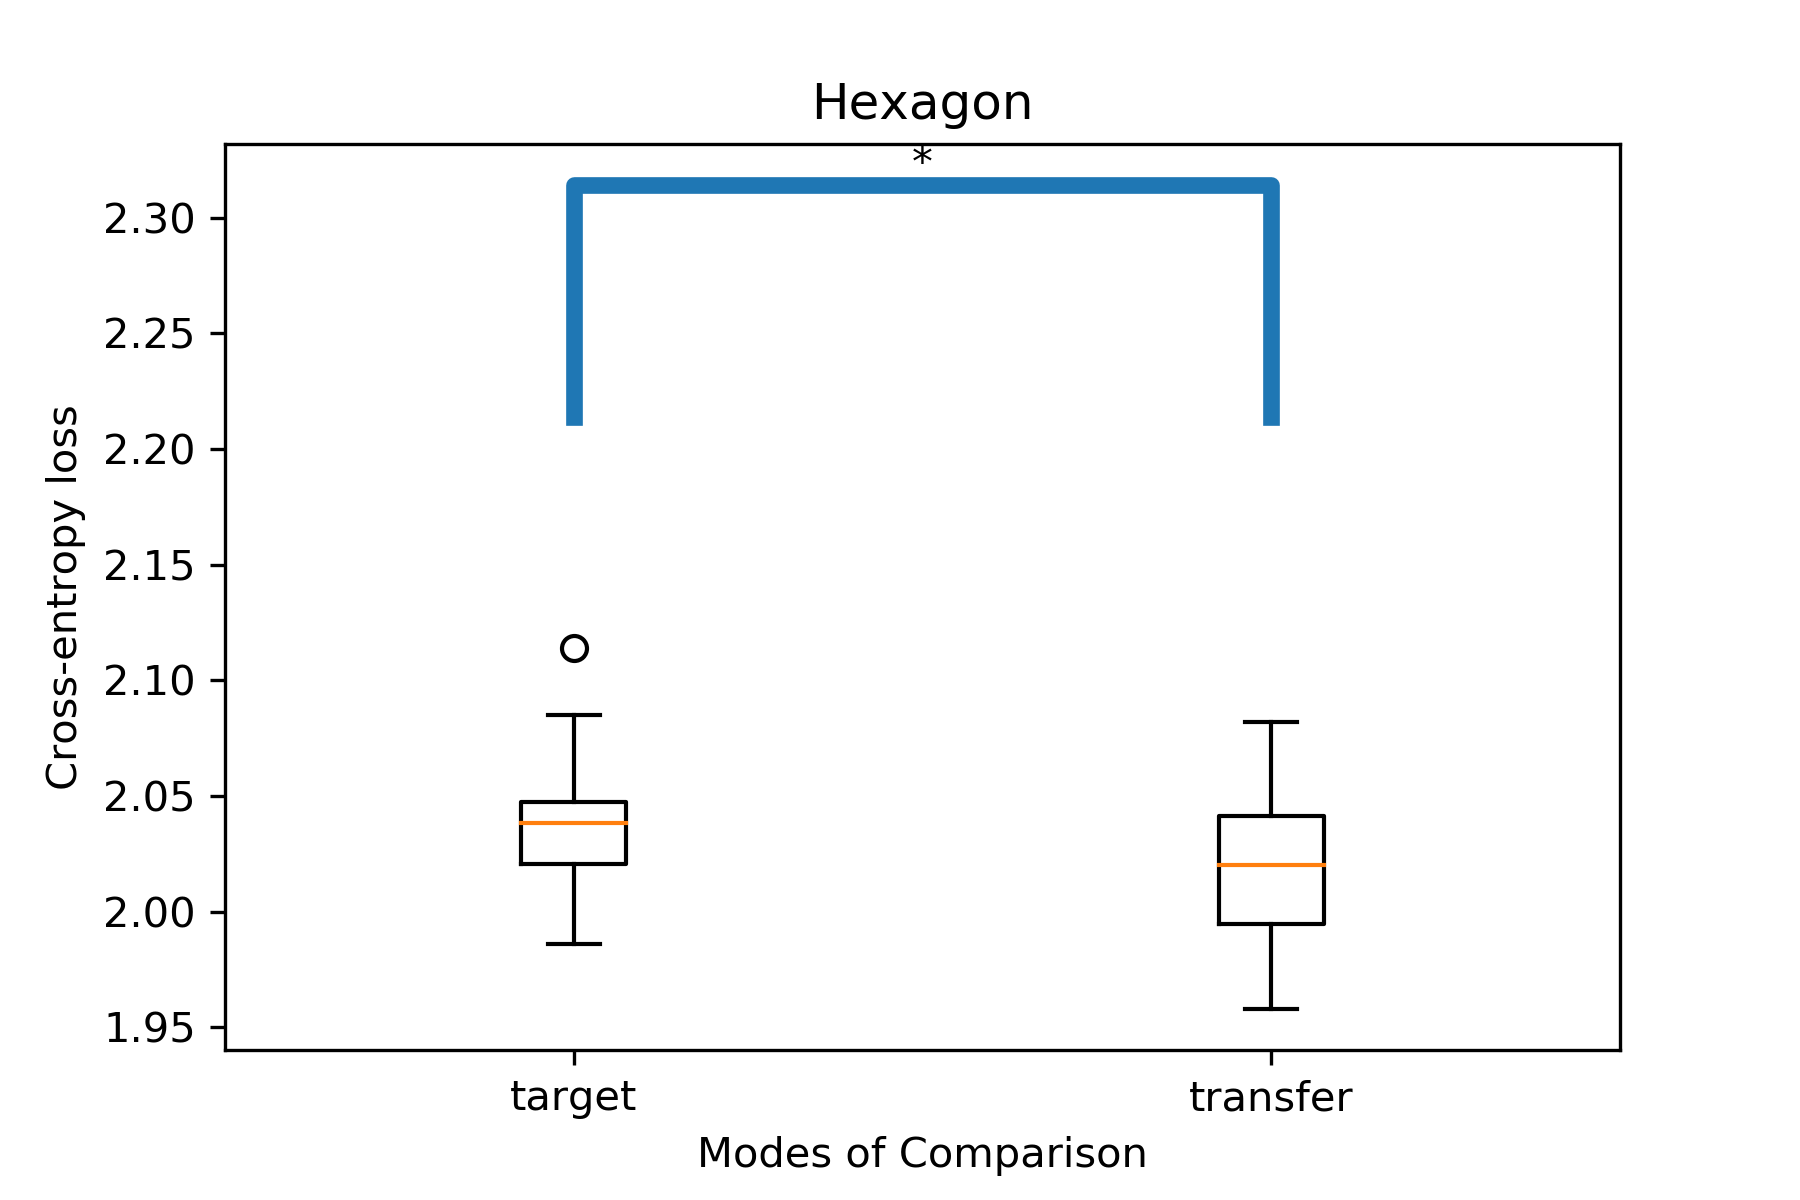
\includegraphics[width=0.31\textwidth]{images/sota/quickdraw_results/hex_ce.png}\quad
            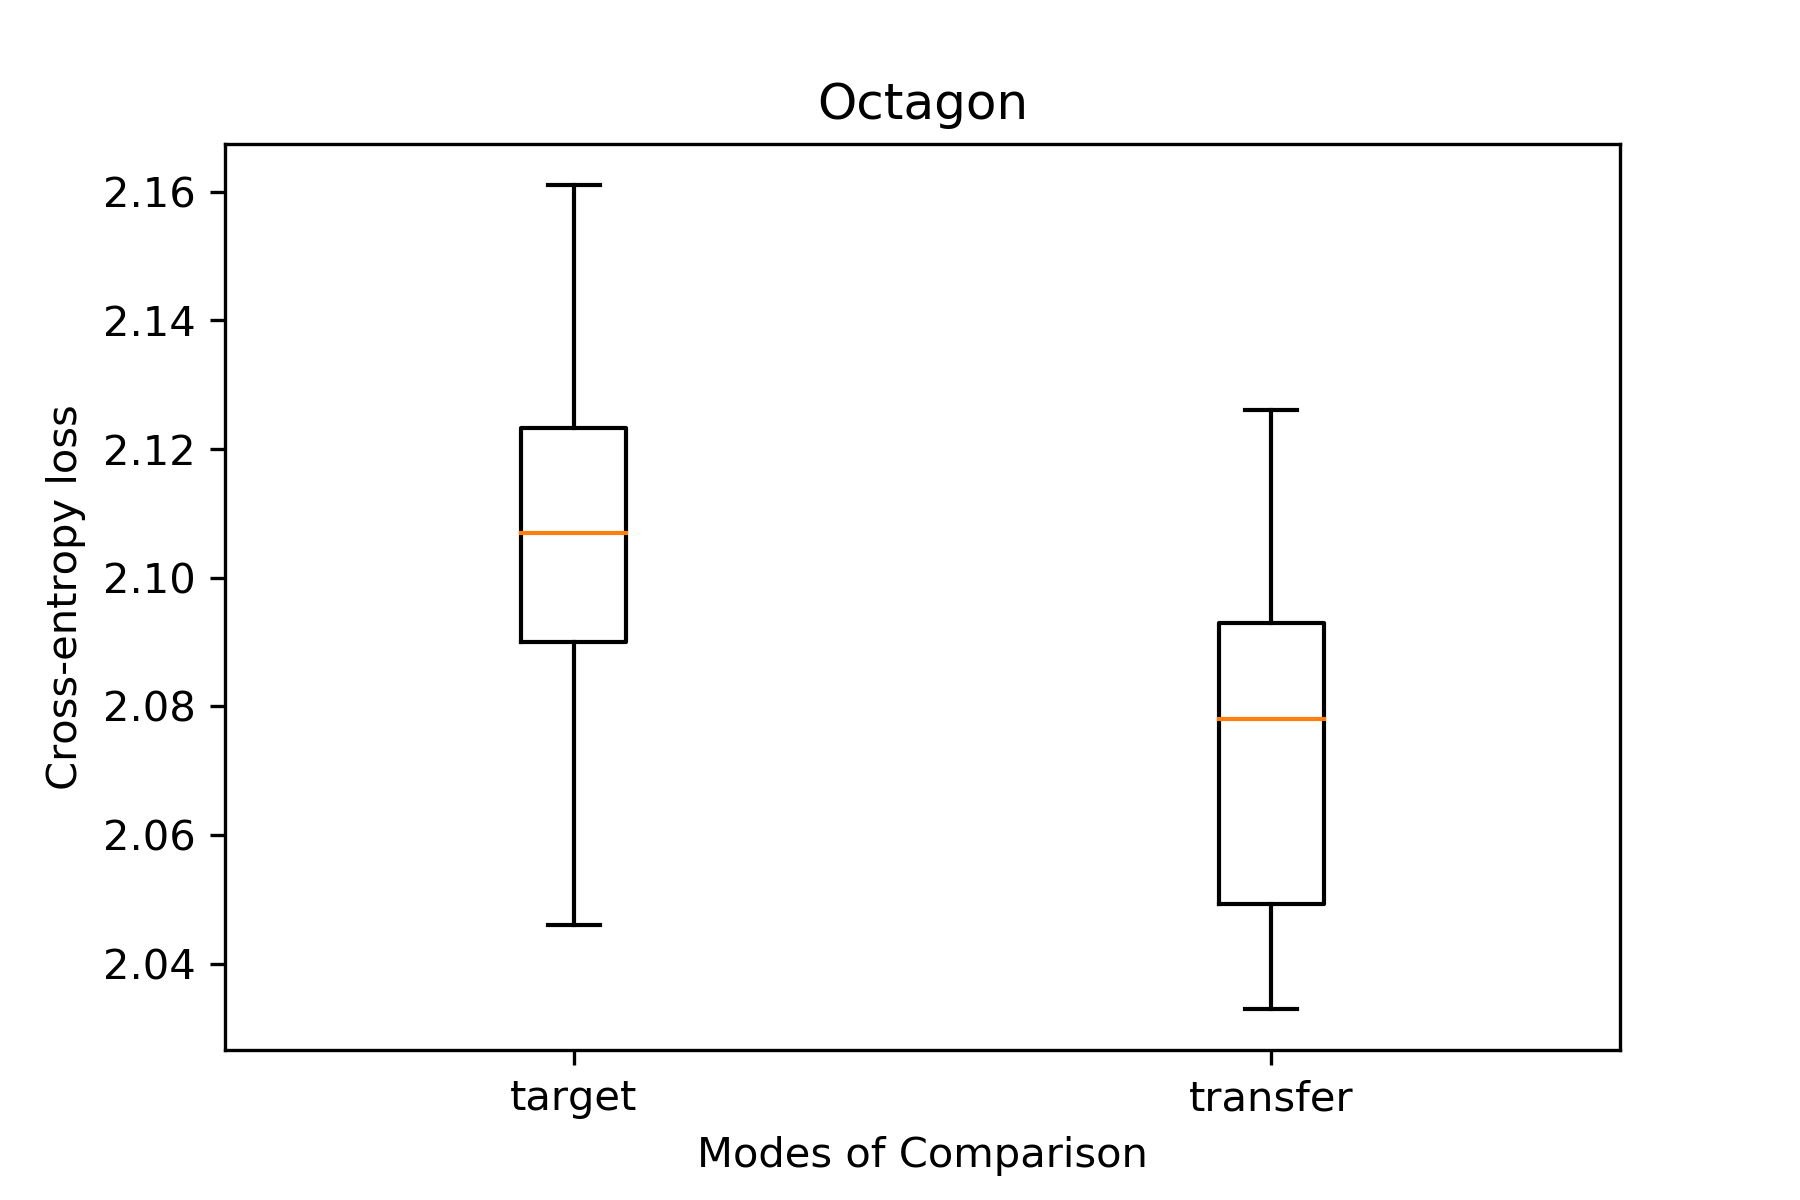
\includegraphics[width=0.31\textwidth]{images/sota/quickdraw_results/oct_ce.png}\quad
          \caption{\textit{QuickDraw!} - crossentropy of prediction of test dataset for different combinations of source/target tasks, with 30 repetitions. We can see that, in all possible source/target task combinations, the transfer learning gives better advantage than just learning from scratch on the target task.}
          \label{fig:quickdraw_crossentropy}
        \end{sidewaysfigure}

      \paragraph{BLEU score}
        The bleu score results are summarized in table \ref{table:bleu_score_quickdraw_transfer}. Transfer learning continusly outperforms the baseline models in this case.

        \begin{table}[!htbp]
          \centering
          \begin{tabular}{|l||c|c|c||c|c|c|}
            \hline
            \multicolumn{1}{|c||}{Aspect/Feature} & \multicolumn{3}{c||}{ Speed } & \multicolumn{3}{c|}{ Freeman }   \\ \hline
            Model / B-score      & B-1  & B-2  & B-3           & B-1  & B-2   & B-3              \\ \hline
            Circle-transfer &    59.0 & 54.5 & 49.6 & 60.0 & 54.7 & 48.9 \\\hline
            Circle-baseline &    70.4 & 65.5 & 60.3 & 65.0 & 58.1 & 50.6 \\\hline

            Trianlge-baseline &  47.3 & 40.0 & 32.6 & 33.2 & 28.2 & 24.0  \\\hline
            Trianlge-transfer &  61.3 & 52.4 & 44.1 & 50.6 & 44.8 & 39.8  \\\hline

            Square-baseline &    46.8 & 40.1 & 32.7 & 44.0 & 39.1 & 34.9  \\\hline
            Square-transfer &    57.9 & 50.8 & 42.9 & 53.0 & 47.4 & 42.3 \\\hline

            Hexagon-baseline &   58.1 & 50.4 & 41.4 & 45.4 & 40.3 & 35.9   \\\hline
            Hexagon-transfer &   62.0 & 54.0 & 44.8 & 47.6 & 42.3 & 37.8  \\\hline

            Octagon-baseline &   55.2 & 47.1 & 38.3 & 43.7 & 38.7 & 34.6   \\\hline
            Octagon-transfer &   57.3 & 49.3 & 40.5 & 46.1 & 41.1 & 36.7  \\\hline

          \end{tabular}
          \caption{\textit{QuickDraw!}: BLEU score results on the generated letters, for the baseline models (trained on the target task only), and the transfer models (the encoder -- style extractor -- is trained on the source task, while the decoder is trained on the target task). The results show an advantage in using transfer learning.}
          \label{table:bleu_score_quickdraw_transfer}
        \end{table}

      \paragraph{End of Sequence analysis}
        Table \ref{table:quickdraw_eos_transfer} summarize the results on end-of-sequence analysis in case of quickdraw. The benefits of transfer learning are clear.
        \begin{table}[!htbp]
          \centering
          \begin{tabular}{|l|c|c|}
          \hline
          Models & Krippendorff coefficient\\ \hline
          Circle-baseline &  0.591 \\ \hline
          Circle-transfer &  0.843 \\ \hline
          Trianlge-baseline & -0.056 \\ \hline
          Trianlge-transfer & 0.609 \\ \hline
          Square-baseline &  0.037 \\ \hline
          Square-transfer &  0.35 \\ \hline
          Hexagon-baseline &  0.07 \\ \hline
          Hexagon-transfer &  0.203 \\ \hline
          Octagon-baseline &  0.073 \\ \hline
          Octagon-transfer &  0.158 \\ \hline

          \end{tabular}
          \caption{\textit{QuickDraw!}: Krippendorff correlation coefficients for the end-of-sequence distributions between the generated letters and the ground truth letters.}
          \label{table:quickdraw_eos_transfer}
        \end{table}

      \paragraph{Strokes analysis}
        Table \ref{table:quickdraw_strokes_transfer} summarize the results on strokes analysis in case of quickdraw. The benefits of transfer learning are clear. We also report the confusion matrix for the strokes, figure \ref{fig:quickdraw_strokes_cnf}. It is notable that the performance of the system in general decreases, as the diversity in the number of strokes increase. But still, transfer learning provides the better results.

        \begin{table}[!htbp]
          \centering
          \begin{tabular}{|l|c|c|}
          \hline
          Models & Krippendorff coefficient\\ \hline
          Circle-baseline &  -0.037 \\ \hline
          Circle-transfer &  0.096 \\ \hline
          Trianlge-baseline & -0.038 \\ \hline
          Trianlge-transfer & 0.419 \\ \hline
          Square-baseline &  0.031 \\ \hline
          Square-transfer &  0.25 \\ \hline
          Hexagon-baseline & -0.084 \\ \hline
          Hexagon-transfer & 0.231 \\ \hline
          Octagon-baseline & 0.055 \\  \hline
          Octagon-transfer & 0.184 \\ \hline

          \end{tabular}
          \caption{\textit{QuickDraw!}: Krippendorff correlation coefficients for the strokes distributions between the generated letters and the ground truth letters.}
          \label{table:quickdraw_strokes_transfer}
        \end{table}

    % Strokes conf matrix
    \begin{figure}[!htbp]
      \centering
      \begin{subfigure}[tb]{0.45\textwidth}
          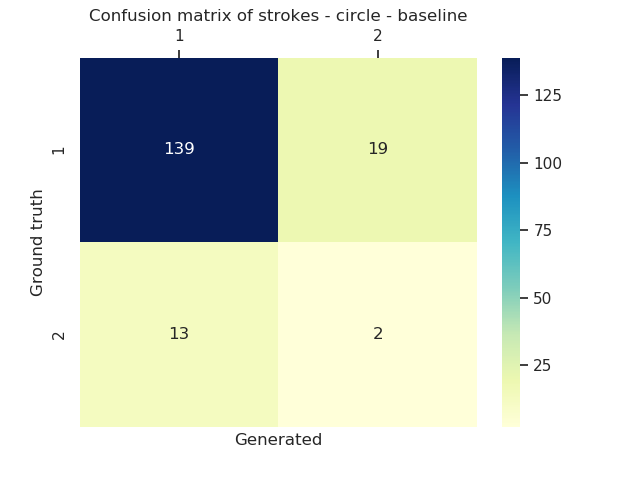
\includegraphics[width=\textwidth]{images/sota/quickdraw_results/quickdraw_circle_target_strokes_heatmap.png}
      \end{subfigure}
      ~
      \begin{subfigure}[tb]{0.45\textwidth}
          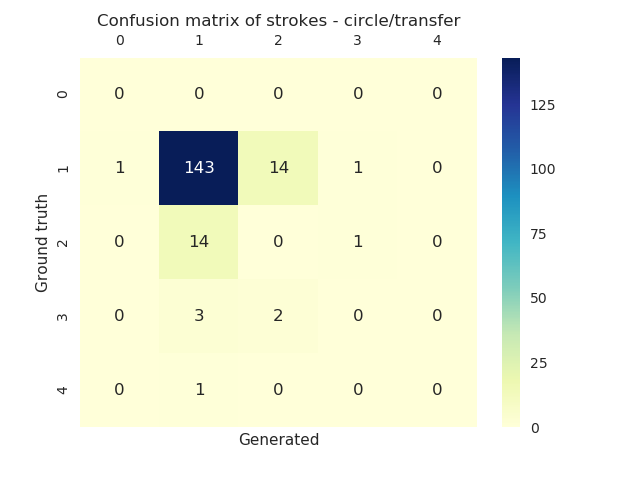
\includegraphics[width=\textwidth]{images/sota/quickdraw_results/quickdraw_circle_transfer_strokes_heatmap.png}
      \end{subfigure}

      ~
      \begin{subfigure}[tb]{0.45\textwidth}
          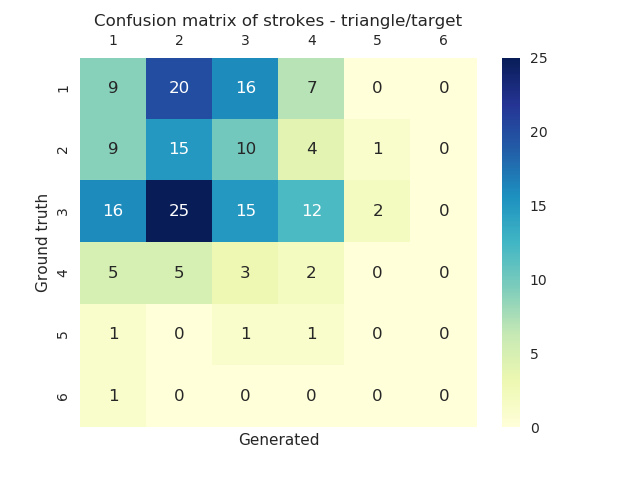
\includegraphics[width=\textwidth]{images/sota/quickdraw_results/quickdraw_triangle_target_strokes_heatmap.png}
      \end{subfigure}
      ~
      \begin{subfigure}[tb]{0.45\textwidth}
          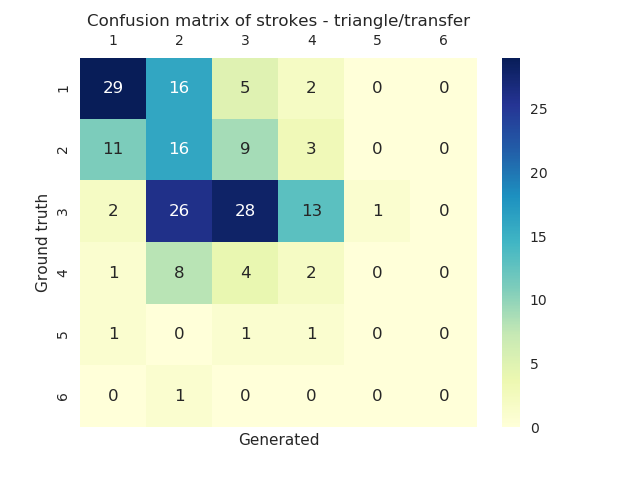
\includegraphics[width=\textwidth]{images/sota/quickdraw_results/quickdraw_triangle_transfer_strokes_heatmap.png}
      \end{subfigure}

      ~
      \begin{subfigure}[tb]{0.45\textwidth}
          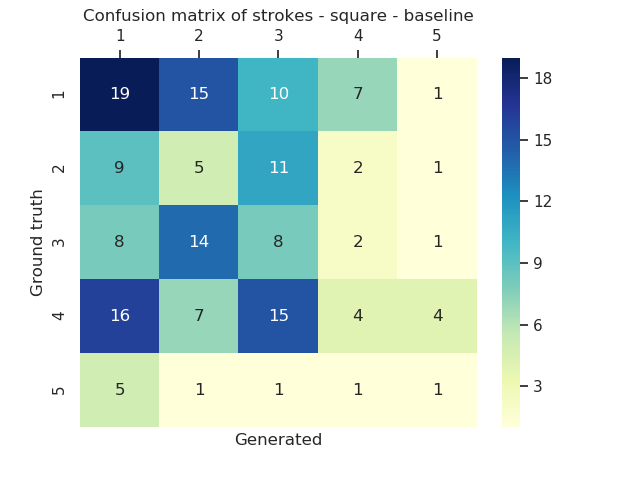
\includegraphics[width=\textwidth]{images/sota/quickdraw_results/quickdraw_square_target_strokes_heatmap.png}
      \end{subfigure}
      ~
      \begin{subfigure}[tb]{0.45\textwidth}
          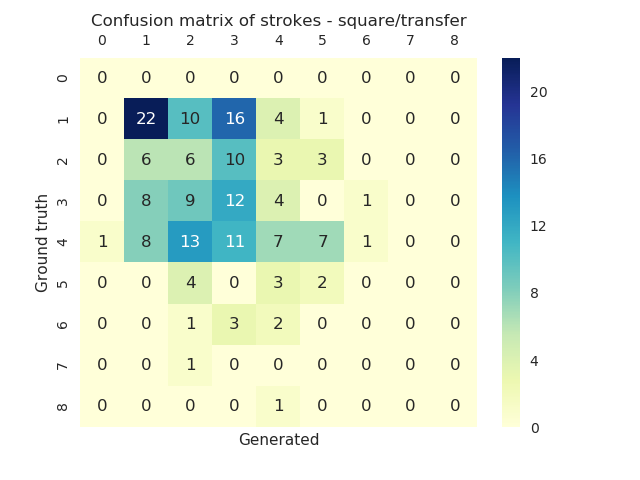
\includegraphics[width=\textwidth]{images/sota/quickdraw_results/quickdraw_square_transfer_strokes_heatmap.png}
      \end{subfigure}

    \end{figure}

    % Strokes conf matrix - continue
    \begin{figure}[!htbp]\ContinuedFloat

      \begin{subfigure}[tb]{0.45\textwidth}
          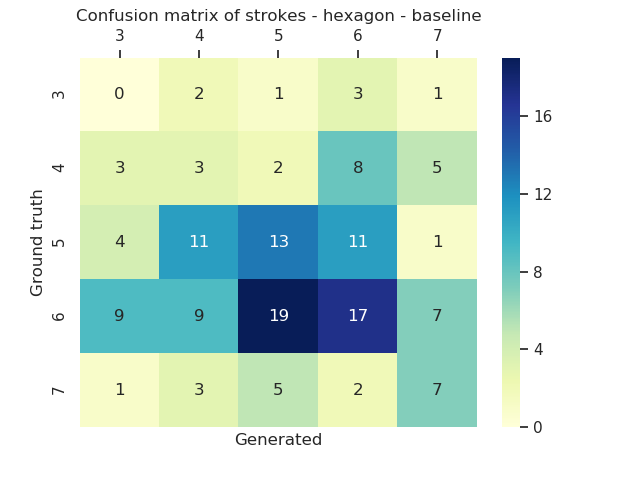
\includegraphics[width=\textwidth]{images/sota/quickdraw_results/quickdraw_hexagon_target_strokes_heatmap.png}
      \end{subfigure}
      ~
      \begin{subfigure}[tb]{0.45\textwidth}
          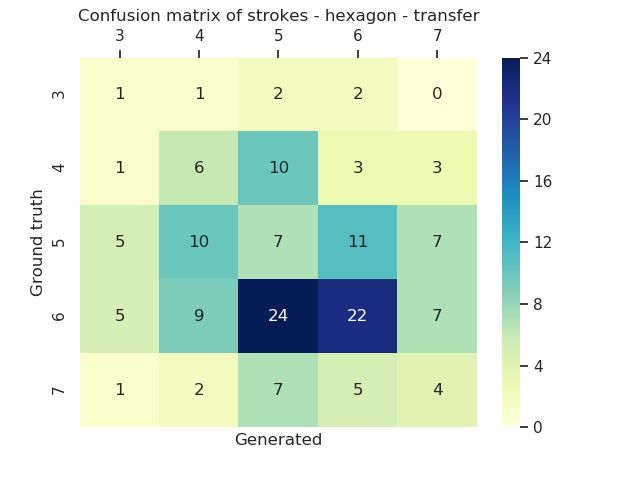
\includegraphics[width=\textwidth]{images/sota/quickdraw_results/quickdraw_hexagon_transfer_strokes_heatmap.png}
      \end{subfigure}

      ~
      \begin{subfigure}[tb]{0.45\textwidth}
          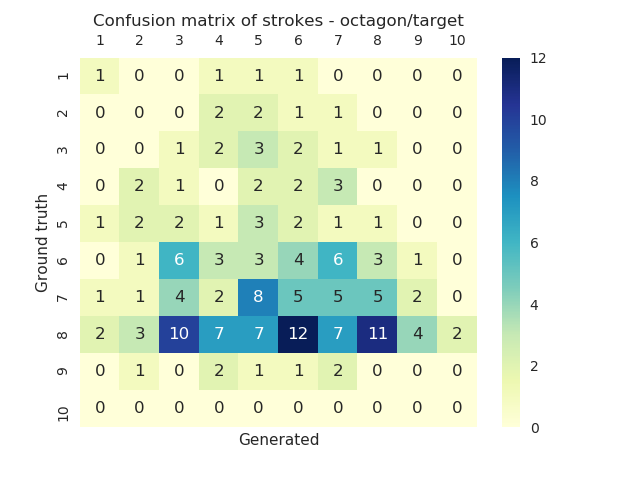
\includegraphics[width=\textwidth]{images/sota/quickdraw_results/quickdraw_octagon_target_strokes_heatmap.png}
      \end{subfigure}
      ~
      \begin{subfigure}[tb]{0.45\textwidth}
          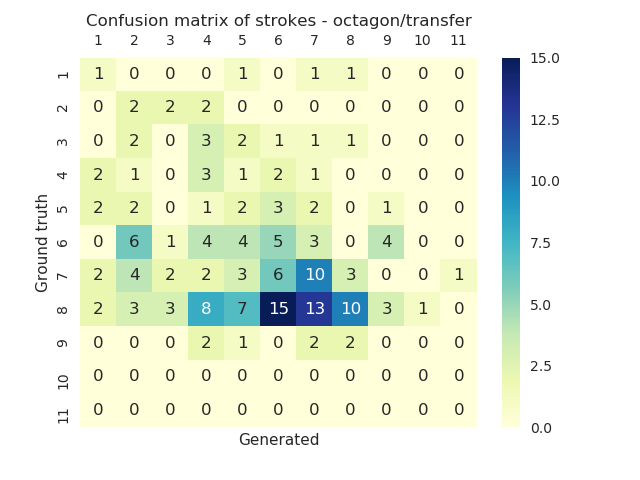
\includegraphics[width=\textwidth]{images/sota/quickdraw_results/quickdraw_octagon_transfer_strokes_heatmap.png}
      \end{subfigure}

      \caption{QuickDraw! Confusion matrix for strokes for both baseline and transfer modes, on the different tasks.}
      \label{fig:quickdraw_strokes_cnf}
    \end{figure}


\section{Summary and take-away message}
\par In this chapter, we presented our hypotheses for style transfer learning. We presented our proposed approach, and the proposed experimental protocol in order to investigate these hypotheses. To have better support for our conclusions, we carried out the experiments on two different datasets, \textit{IRONOFF} and \textit{QuickDraw!}, both of them presenting different challenges and behviors: \textit{IRONOFF} has more clear semantics, made by a pen, while in \textit{QuickDraw!} the contributors excerted more freedom on their work, and most of the work is believed to be done by the mouse or a tablet. Also, we chose to perform the study on the worst case scenario, where there is an abundance of data available to the target task. To better understand and compare transfer learning versus the baseline models (models trained only on the target task), we considered multiple performance metrics: the loglikelihood of prediction, the BLEU score, end-of-sequence and strokes analyses for the generated shapes.

\par The results overwhelmingly point to the benefit of transfer learning compare to the baselines on the different proposed metrics, thus providing a strong evidence to our hypotheses.